\begin{flushleft}
    \large
    \section{Design}
        \subsection{Programming Language and Libraries}
            I chose Python for my chosen Programming Language, it's very versatile, and I have lots of experience with the language
            already. It's great for rapid prototyping which I feel is necessary for a project of this scale. I already used it for 
            my prototype, so I will be able to reuse some parts of my previous code base. Such as my Matrix and WorldMap Class'. \\
            \vspace{0.2cm}
            Below is a list of key libraries I will be using in my project: \\
            \subsubsection*{Pygame}
            Pygame is a highly customizable and well-developed binding of \textit{Simple DirectMedia Layer} (SDL) Library. 
            It has a full set of 2d drawing tools, along with keyboard and audio capabilities. I have lots of experience with Pygame, so 
            I already have code which I can take from, which will speed up development when dealing with the Pygame library. \\
            \vspace{0.2cm}
            I will be using Pygame to graphically display the Environment I create as part of my Technical Solution. This
            will be done in a way similarly to my prototype, displaying each tile as a specified colour. Pygame is purely a 
            method to graphically output the current state of the simulation. \\
            \vspace{0.2cm}
            This will be used to fulfil the whole of \textbf{Objective 2} \\
            \subsubsection*{JSON}
            The ability to load JSON Formatted Files is a key part of my User Input and overall Technical Solution. The JSON 
            Library in Python allows this with relative ease, along with saving JSON data where needed. I will be using JSON files
            to store the User Inputted Parameters to the program. These parameters will be things like the size of the Simulation, and 
            Neural Network Structure. \\
            \vspace{0.2cm}
            This will be used to fulfil parts of \textbf{Objective 1}, more specifically \textbf{Objectives 1.1, 1.3, 1.5} \\
            \subsubsection*{Pickle}
            Pickle will be used to write Binary Files with Python. You can use it to save objects, such as classes
            or lists, and load them. I will be using pickle to store the Matrix Class when saving the Training Progress of
            the Neural Network. Each Weight and Bias will need to be stored in order to resume the exact training position of the
            Network. I will also be storing states for Experience Replay, and the Data Points for plotting Training Data. \\
            \vspace{0.2cm}
            This will be used to fulfil \textbf{Objectives 5.11, 7.4, 8.1} \\
            \subsubsection*{MatPlotLib}
            MatPlotLib is a simple way to visualize Numerical data. You can very easily plot graphs from a set of
            data points. With my Technical Solution I intend to load data previously stored with Pickle, and plot it with this Library. \\
            \vspace{0.2cm} 
            This will be used to fulfil \textbf{Objective 8.3} \\
        \subsection{High Level Overview}
            \large
            The main purpose of the project is to answer my investigations question. I'm answering this question by developing 
            a program which simulates an Environment in which a Machine Learning Algorithm can Explore and Interact with. The user
            will be able to alter the parameters of this Machine Learning Algorithm and Simulation in order to test different aspects. 
            This will be done through a JSON File in which the listed parameters will have specified ranges they must be between. The
            Descriptions and Ranges of these Parameters are shown under the File Structure Section. \\
            \vspace{0.2cm}
            The Machine Learning Algorithm will be Deep Q Learning, utilising a Dual Neural Network at its core. A Dual Neural Network
            is formed from 2 Neural Networks, a Main and Target. Within Deep Q Learning we are updating a guess with a guess,
            this leaves us with instability. To solve this, the Target Network is a copy of the Main Network, made every $N$ Steps, and is used to 
            inform the Bellman Equation (mentioned in Modelling of the Problem) when calculating Expected Values in the Loss Function. 
            Below is shown a diagram of how a Dual Neural Network functions: \\
            
            \vspace{0.5cm}
            \centerline{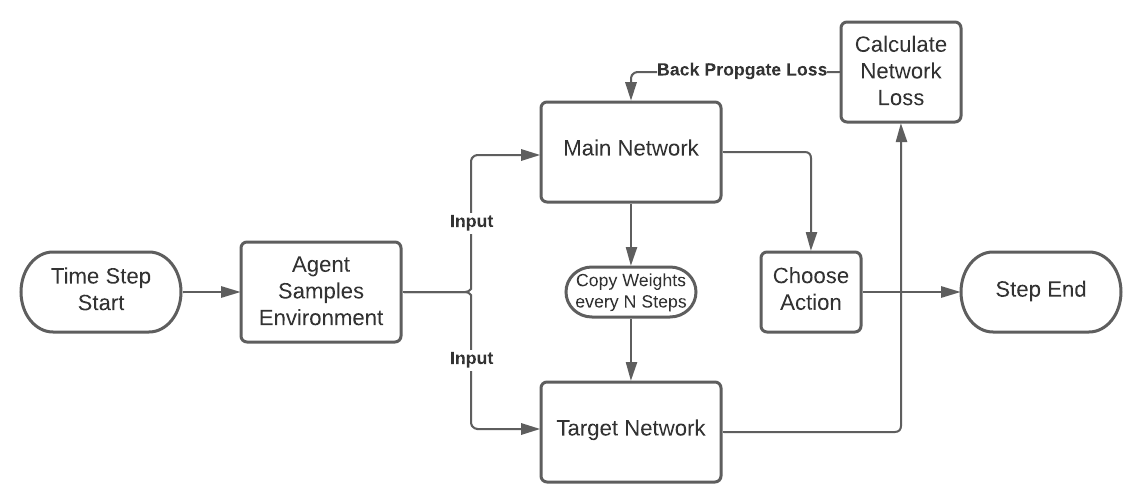
\includegraphics[width=\textwidth]{Images/Design/DualNetwork.png}}
            \vspace{0.5cm}

            The simulated environment will be procedurally generated using Perlin Noise and Poisson Disc Sampling. Perlin Noise will
            generate a Height Map of values, these values will then get mapped to colour bands (which are specified by the User). Poisson
            Disc Sampling will be used to place Items around the Environment which the Agent will be able to interact with through an Action.
            The Terrain and Items will be displayed to the screen via a Window, similar to my prototype like this: \\

            \begin{figure}[H]
                \centering
                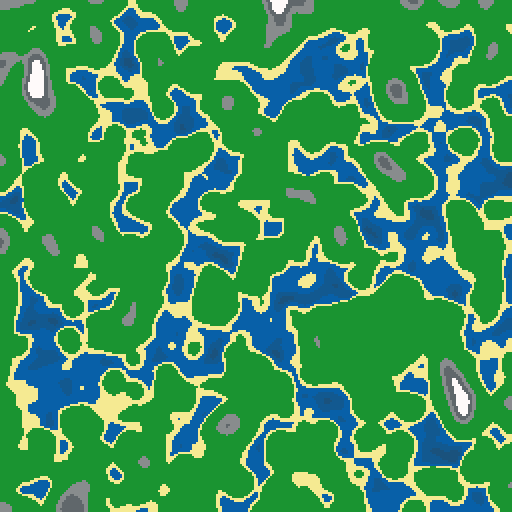
\includegraphics[width=8cm]{Images/Prototype/Seed420 Colour.png}
                \caption*{Terrain Generated by my Prototype}
            \end{figure}

            Within the simulated environment are generated Enemies which path find towards the Agent in an attempt to hinder the Agents
            survival. This can be done using a simple pathfinding algorithm. If these enemies are ever to touch Water, they will die. 
            The Agent will be a character controlled within the environment by the Deep Q Learning Algorithm, which has a specific set
            of Actions. Upon picking an action the Agent will be rewarded or penalized depending on which action is picked in which state. If the
            Agent is ever in a Water Tile or within an Enemy, the Agent will be penalized, and the environment will be generated again.

            To pick the Agents Action the surrounding Terrain is sampled for Greyscale Colour Values. These Greyscale values are then 
            passed into the Main Neural Network to inform the decision. With the use of the SoftMax Logistics Function, we can generate a 
            probability distribution from the Neural Network outputs. \\
            \vspace{0.2cm}
            With the use of a training method called Epsilon Greedy we can balance Exploration and Exploitation. Epsilon is defined as
            a value at the start of the Training Session, and is slowly multiplied by a regression value each step. When picking an action
            a Random Number is generated between 0 and 1, and then compared with the Epsilon Value. If the random value is less than Epsilon
            we pick a random Action, Exploration. If the random value is greater than Epsilon we use an informed decision, Exploitation. \\
            \vspace{0.2cm}
            Below is shown a simplified Flow Chart of the whole process: \\
            
            \vspace{0.5cm}
            \centerline{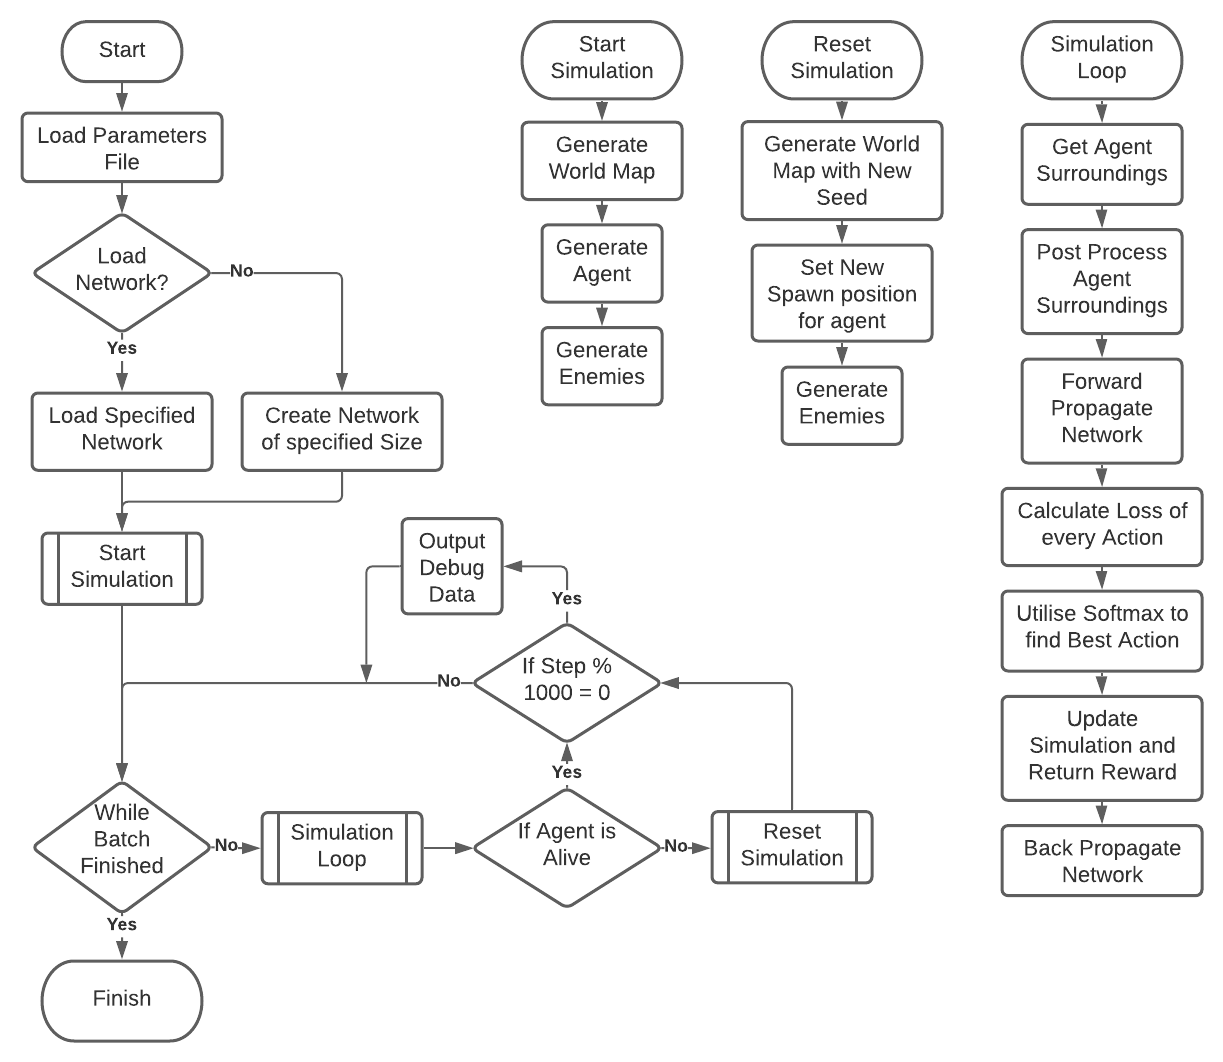
\includegraphics[width=\textwidth]{Images/Design/NEAFlowChart.png}}
            \vspace{0.5cm}
        \subsection{User Interface/Graphical Output Design}
            The Graphical Output for the Program will be a display the current environment as a Grid of Coloured Tiles. I have previously
            implemented the display of a Grid of Tiles in my Prototype, but I want to expand this to include a Debug Menu at the side.\\
            \vspace{0.2cm}
            The Debug Menu will be enabled through the JSON File, and will display the Neural Network Activations as greyscale values. 
            It will scale to the size of the Network, and will be helpful for debugging. Below is shown a UI Screenshot from the final
            build: \\

            \begin{figure}[H]
                \centering
                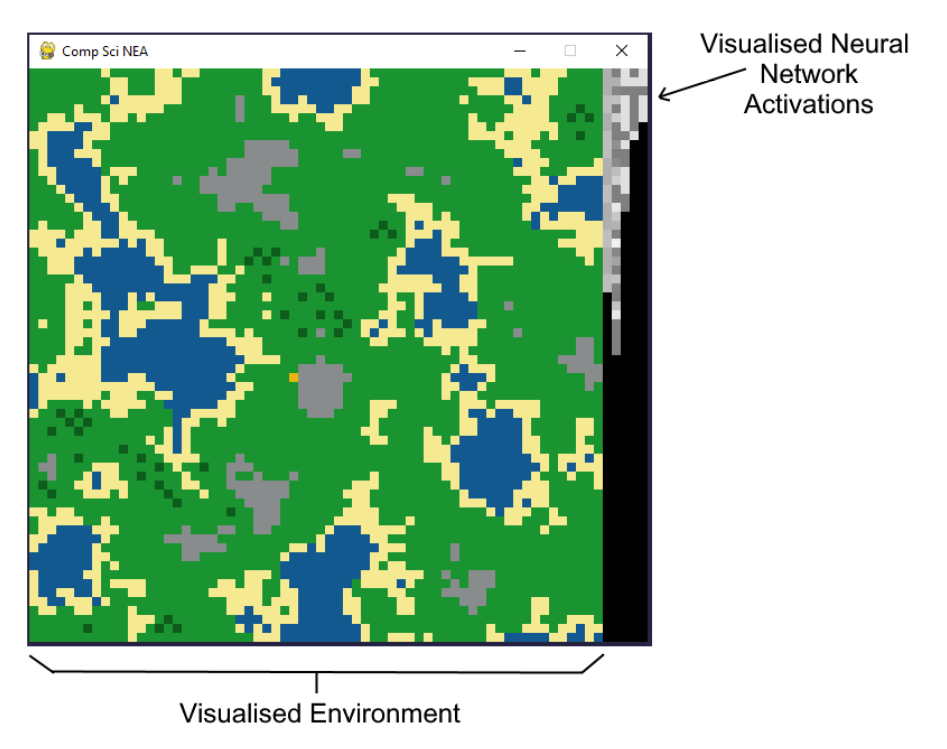
\includegraphics[width=14cm]{Images/Design/AnnotatedUIExample.PNG}
            \end{figure}
        \subsection{Agent Interaction and Reward Design}
            The Agent's interaction with the Algorithm and Simulation is very important. If designed incorrectly the Algorithm will be unable 
            to grasp the Simulation Properly. \\
            \vspace{0.2cm}
            The Agent will sample the surrounding environment for Greyscale colour values of each Tile. This Greyscale data will then be
            converted into a Vector to utilise it as the Neural Networks input. This works well because Greyscale Values are a value 
            from $0\to 1$, values like this are often used as Neural Network inputs. Below I have marked the Greyscale values (1 Decimal Place)
            on each of the colours from a sample situation. The colour conversion will be done using a simple algorithm which is shown later
            in Design under Description of Algorithms.

            \begin{center}
                \begin{tabular}{m{0cm} C{1cm} C{1cm} C{1cm} C{1cm} C{1cm}}
                        \rule{0pt}{1.2cm}% %
                        &\cellcolor{Water}0.3 & \cellcolor{Water}0.3 & \cellcolor{Beach}0.9 & \cellcolor{Grass}0.4 & \cellcolor{Enemy}0.2 \\
                        \rule{0pt}{1.2cm}% %
                        &\cellcolor{Water}0.3 & \cellcolor{Beach}0.9 & \cellcolor{Grass}0.4 & \cellcolor{Grass}0.4 & \cellcolor{Grass}0.4 \\
                        \rule{0pt}{1.2cm}% %
                        &\cellcolor{Beach}0.9 & \cellcolor{Grass}0.4 & \cellcolor{Player}0.7 & \cellcolor{Grass}0.4 & \cellcolor{Grass}0.4 \\
                        \rule{0pt}{1.2cm}% %
                        &\cellcolor{Grass}0.4 & \cellcolor{Grass}0.4 & \cellcolor{Grass}0.4 & \cellcolor{Grass}0.4 & \cellcolor{Tree}0.2 \\
                        \rule{0pt}{1.2cm}% %
                        &\cellcolor{Tree}0.2  & \cellcolor{Grass}0.4 & \cellcolor{Grass}0.4 & \cellcolor{Grass}0.4 & \cellcolor{Grass}0.4 \\
                \end{tabular}
            \end{center}

            The Agent will have a specific set of actions it can use at any time to interact with the Environment. These actions may be good
            or bad given each individual situation, that is for the Algorithm to try and decipher through the gains and loss' of Reward. Below
            is shown a table of actions the Agent will utilise. I designed this action set to be relatively simple as to keep the complexity of the
            Simulation as little as possible. 

            \vspace{0.2cm}
            \begin{center}
                \begin{tabular}{| c | c | c |}
                    \hline
                    Action No. & Action Name & Action Description \\
                    \hline
                    1 & Move Up & Agent Moves Up one Tile \\
                    \hline
                    2 & Move Right & Agent Moves Right one Tile \\
                    \hline
                    3 & Move Down & Agent Moves Down one Tile \\
                    \hline
                    4 & Move Left & Agent Moves Left one Tile \\
                    \hline
                    5 & Pickup Item & The Item on the same Tile as the Agent is collected \\
                    \hline
                    6 & Attack & Enemies within a radius of the Agent are attacked \\
                    \hline
                    7 & Noop & Null Action / No Action performed \\
                    \hline
                \end{tabular}
            \end{center}
            \vspace{0.2cm}
            
            The Reward Structure for a given Situation is very important, if the Agent is being rewarded incorrectly this could lead to drastic
            issues with training and calculating expected values. I decided to focus my Reward Structure on Exploration and Motivating the Agent
            to collect Items while also rewarding successfully eliminating Enemies. This was based off of feedback which was given to me by my
            Expert in my second Interview. Below is shown a table of the individual Reward values I assigned when initially designing my Project.

            \vspace{0.2cm}
            \begin{center}
                \begin{tabular}{| L{2cm} | L{1cm} | L{8cm} |}
                    \hline
                    Reward Name & Value & Reward Description \\
                    \hline
                    Explore Reward & 0.01 & Given to the Agent when it enters a previously unvisited Tile  \\
                    \hline
                    Collect Item Reward & 1 & Given to the Agent when it collects an Item \\
                    \hline
                    Attack Reward & 0.5 & Given to the Agent upon a successful Attack \\
                    \hline
                    Attack Failed Reward & -0.1 & Given to the Agent when an Attack has failed \\
                    \hline
                    Death Reward & -1 & Given to the Agent when it is killed \\
                    \hline
                \end{tabular}
            \end{center}
            \vspace{0.2cm}

            Shown below is shown a Diagram with the appropriate reward values for each Tile in the sample situation. Along with a flow chart 
            detailing the steps it takes to calculate the reward of a given Action taken by the Agent. All reward gained during the flow process is
            added to a total and returned as part of the Reward Function.

            \begin{center}
                \begin{tabular}{m{0cm} C{1cm} C{1cm} C{1cm} C{1cm} C{1cm}}
                        \rule{0pt}{1.2cm}% %
                        &\cellcolor{Water}-0.1 & \cellcolor{Water}-0.1 & \cellcolor{Beach}0.01 & \cellcolor{Grass}0.01 & \cellcolor{Enemy}-0.1 \\
                        \rule{0pt}{1.2cm}% %
                        &\cellcolor{Water}-0.1 & \cellcolor{Beach}0.01 & \cellcolor{Grass}0.01 & \cellcolor{Grass}0.01 & \cellcolor{Grass}0.01 \\
                        \rule{0pt}{1.2cm}% %
                        &\cellcolor{Beach}0.01 & \cellcolor{Grass}0.01 & \cellcolor{Player}0 & \cellcolor{Grass}0.01 & \cellcolor{Grass}0.01 \\
                        \rule{0pt}{1.2cm}% %
                        &\cellcolor{Grass}0.01 & \cellcolor{Grass}0.01 & \cellcolor{Grass}0.01 & \cellcolor{Grass}0.01 & \cellcolor{Tree}1 \\
                        \rule{0pt}{1.2cm}% %
                        &\cellcolor{Tree}1  & \cellcolor{Grass}0.01 & \cellcolor{Grass}0.01 & \cellcolor{Grass}0.01 & \cellcolor{Grass}0.01 \\
                \end{tabular}
                \vspace{0.5cm}
                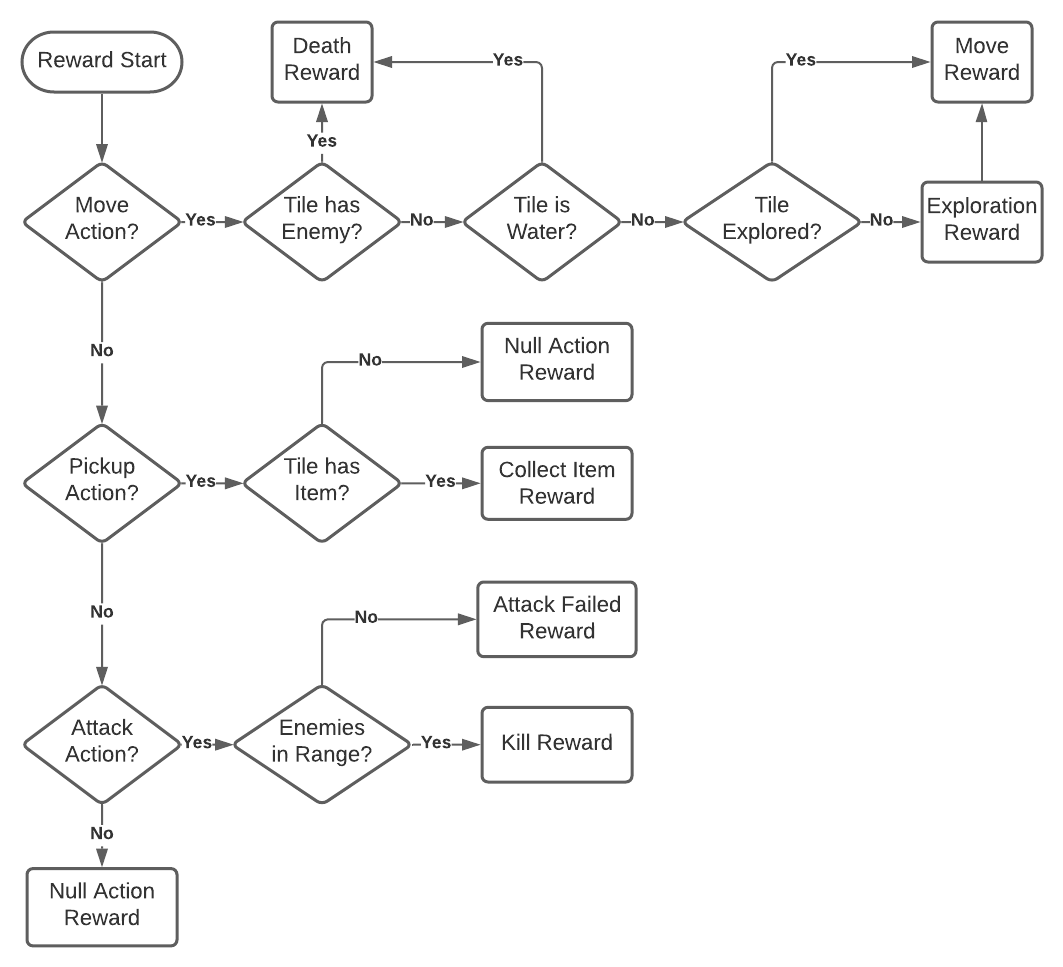
\includegraphics[width=\textwidth]{Images/Design/RewardActionStructure.png}
            \end{center}   
        \subsection{Object Orientated Structure}
            \large
            My project is formed from several classes, each having a specific role. They primarily use composition, due to being tightly linked
            together. Although some links are more similar to aggregation. I designed my project to primarily break down into two parts, the
            Neural Network and the Environment. These are split into three primary classes, which link together through the use of a Management
            class. This management class oversees and organizes all Primary aspects of the program, storing instances of its child classes, and
            passing references to each other through Methods. It also handles the Setup and Resetting for the entire project, if the Agent is killed
            it detects this and will signal the Environment to regenerate, create new enemies set the Agents new spawn position. Below is shown an 
            abstraction of the Full Class Diagram, utilising only the names of the classes due to each class having too many methods to display fully.
            The Full Class Diagram is shown on its own page at the end of this Section.

            \vspace{0.5cm}
            \centerline{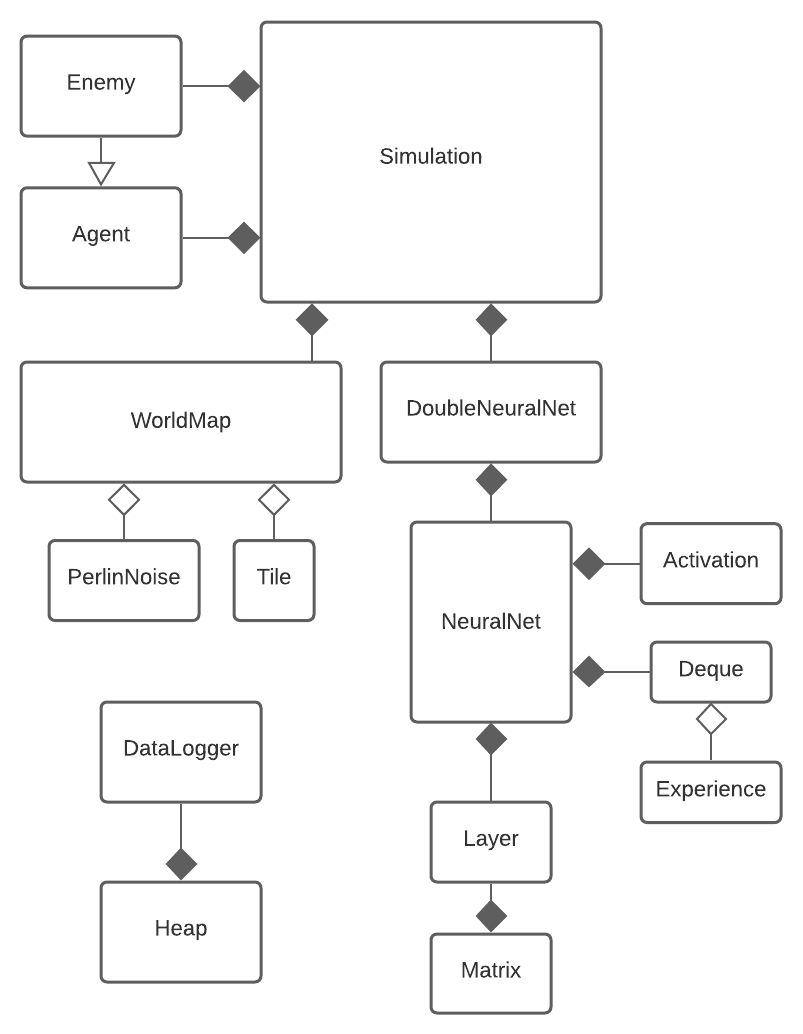
\includegraphics[width=.65\textwidth]{Images/Design/SimplifiedClassDiagram.png}}
            \vspace{0.5cm}

            As you can see from the Class Diagram there is a lot of classes within my project, all linked together in various different ways. 
            Below is shown a more in-depth dive into each Class' Purpose, along with Explanations of their Primary Methods.\\
            \subsubsection{Simulation Class}
                The Simulation Class is the Management Class of the whole Program. This will be instantiated upon the launch of the program, and all user
                interactions with the program will be done through it. The Methods within this class are designed to be very abstracted from the core
                of the program. There are never any direct Matrix Operations or logic performed in this Class except for checking the parameters, and
                basic setup such as instantiating new Enemies \textit{if they are enabled}. It does however call Methods which then run this logic.

                \begin{figure}[H]
                    \centering
                    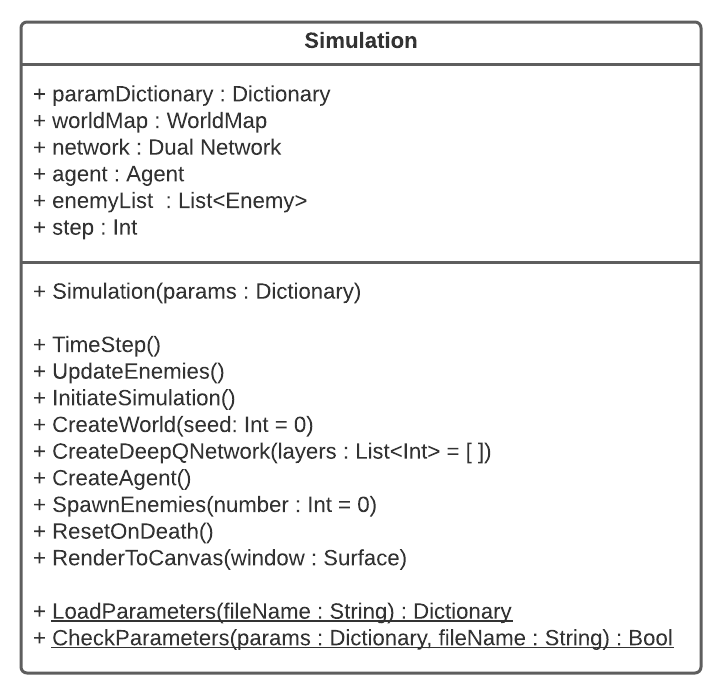
\includegraphics[width=.6\textwidth]{Images/Design/Classes/Simulation.png} 
                    \caption*{The Simulation Class}
                \end{figure}
            \subsubsection{Agent, Enemy and WorldMap Class}
                Both these Classes will be used by the Simulation Class to form the Environment and its interactions. The World Class will host the
                Procedural Generation Methods along with storing any Terrain related data. Perlin Noise and Poisson Disc Sampling are used here to
                generate the Height Map for the Terrain and Generate Objects. The Agent Class is used to interact with the Environment, Methods for 
                Sampling the Tile Data and processing this into Greyscale Values for use in the Dual Neural Network. The Agent also has Reward Methods
                for calculating the Reward when given a certain State and Action. This is shown under the Agent Interaction and Reward Design Section. \\
                \vspace{0.2cm}
                The Enemy Class inherits from the Agent Class, implementing its own Commit Action and Spawn Position Method. This inheritance is so 
                that any Agent Methods which might be needed in the final implementation.
                \vspace{0.2cm}
                This fulfils objectives under \textbf{Objective 4} \\

                \begin{figure}[H]
                    \centering
                    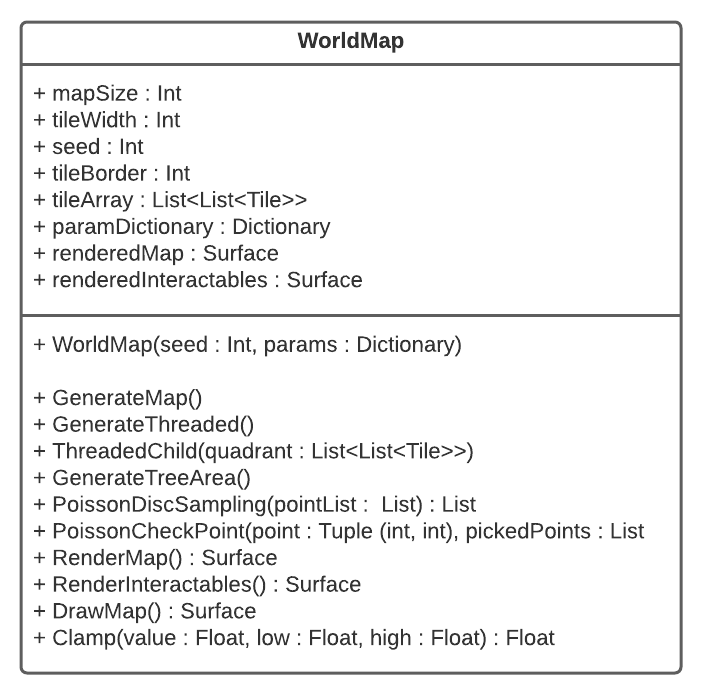
\includegraphics[width=.65\textwidth]{Images/Design/Classes/WorldMap.png}
                    \caption*{The WorldMap Class}
                \end{figure}
                \begin{figure}[H]
                    \centering
                    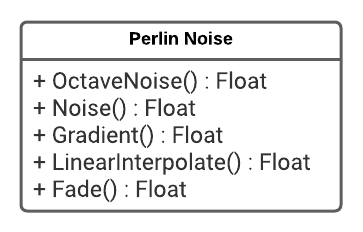
\includegraphics[width=.45\textwidth]{Images/Design/Classes/PerlinNoise.png}
                    \caption*{The PerlinNoise Class}
                \end{figure}
                \begin{figure}[H]
                    \centering
                    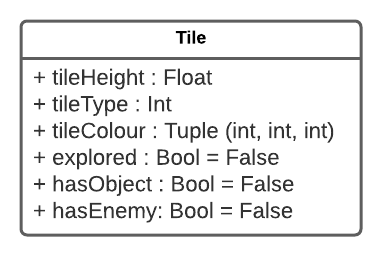
\includegraphics[width=.35\textwidth]{Images/Design/Classes/Tile.png}
                    \caption*{The Tile Class}
                \end{figure}
                \begin{figure}[H]
                    \centering
                    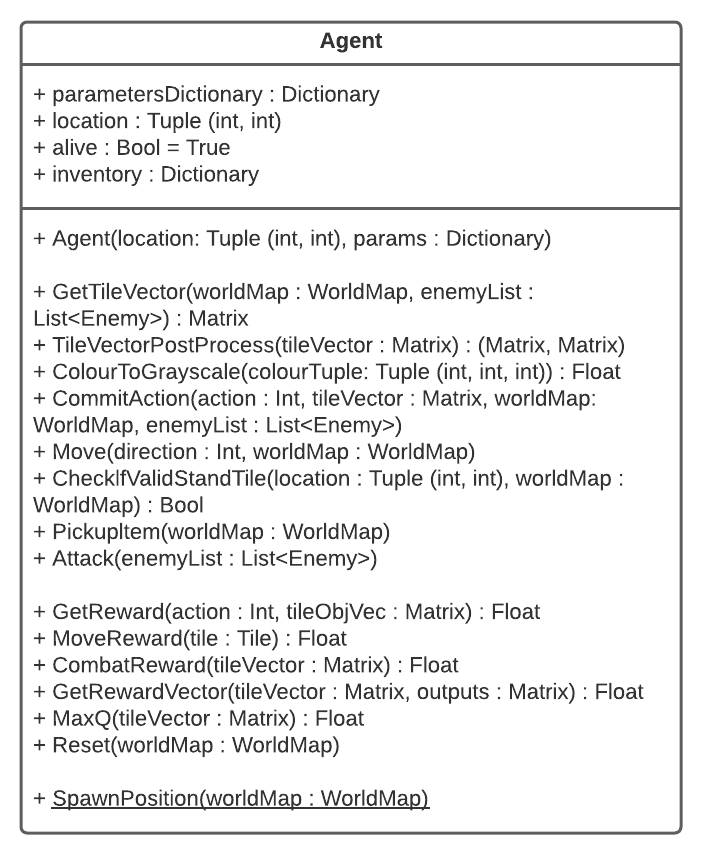
\includegraphics[width=.65\textwidth]{Images/Design/Classes/Agent.png}
                    \caption*{The Agent Class}
                \end{figure}
                \begin{figure}[H]
                    \centering
                    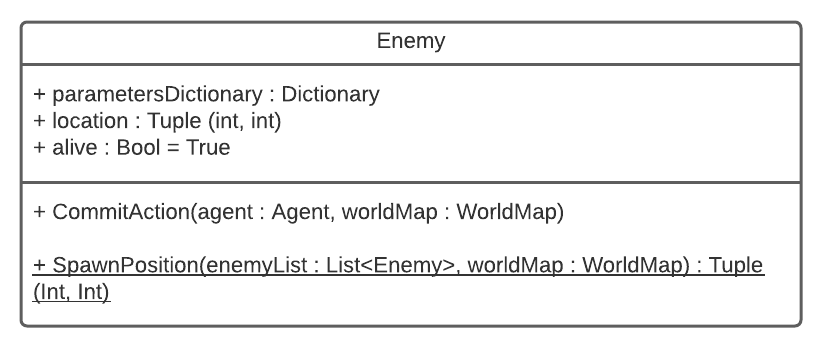
\includegraphics[width=.80\textwidth]{Images/Design/Classes/Enemy.png}
                    \caption*{The Enemy Class}
                \end{figure}
            \subsubsection{DoubleNeuralNet Class Family}
                The DoubleNeuralNet Class is instantiated as part of the setup in Simulation. This class is the parent to both the Main and Target 
                Neural Networks, which are both instances of NeuralNet. DoubleNeuralNet hosts the Top-Level methods for invoking a Time Step
                within the Network. The TimeStep Method will be called from Simulation, into this method is passed references to the current WorldMap
                along with the current Agent. This then Forward Propagates the Main and Target Neural Networks, performs the logic for calculating the
                correct action utilising SoftMax and Epsilon Greedy. The expected values, and subsequently the Loss are calculated, which is then used
                to Back Propagate the Main Network. \\
                \vspace{0.2cm}
                The NeuralNet Class holds a list of Layer Objects, along with intermediate Forward Prop, Back Prop and Update Methods. Upon initialisation
                of the NeuralNet Object, it will create the list of Layers with the specified sizes from the User. The contained Methods simply perform
                the Layer$\to$Layer Logic which is needed for Forward and Back Propagation. \\
                \vspace{0.2cm}
                Each Layer Object holds Weight, Bias, Pre-Activation, and Activation Data. This is all utilised within the Forward and Back Propagation 
                Process. The contained data is all stored in Matrices to speed up calculations. \\
                \vspace{0.2cm}
                This fulfils objectives under \textbf{Objective 5} \\

                \begin{figure}[H]
                    \centering
                    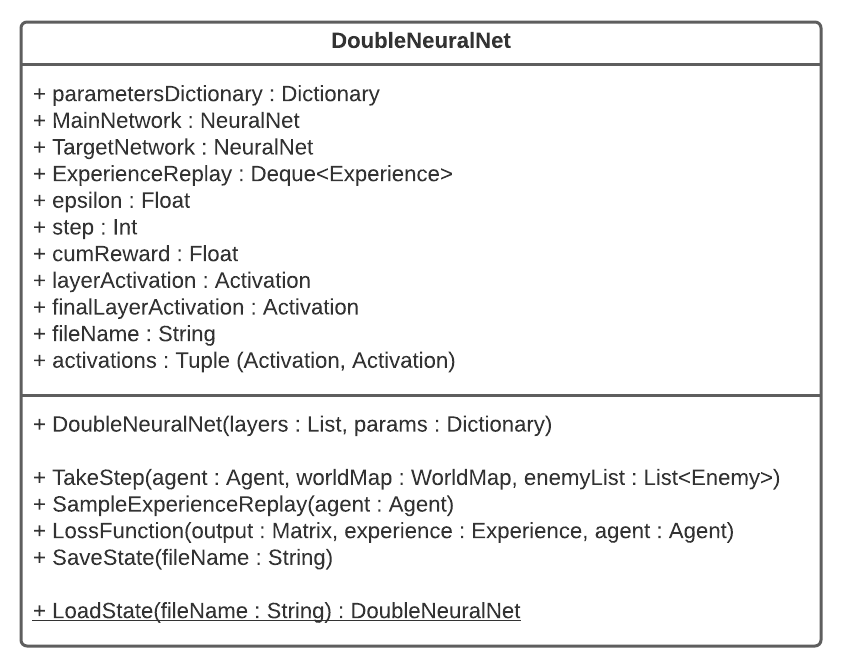
\includegraphics[width=.70\textwidth]{Images/Design/Classes/DoubleNeuralNet.png} 
                    \caption*{The DoubleNeuralNet Class}
                \end{figure}
                \begin{figure}[H]
                    \centering
                    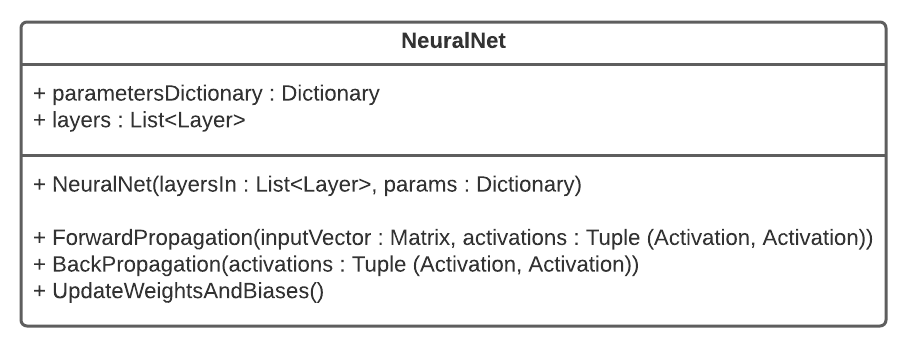
\includegraphics[width=.80\textwidth]{Images/Design/Classes/NeuralNet.png} \\
                    \caption*{The NeuralNet Class}
                \end{figure}
                \begin{figure}[H]
                    \centering
                    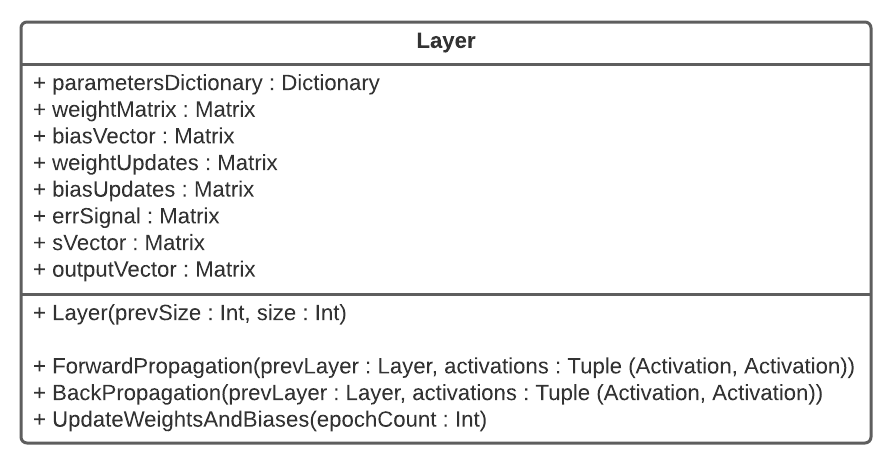
\includegraphics[width=.75\textwidth]{Images/Design/Classes/Layer.png} \\
                    \caption*{The Layer Class}
                \end{figure}
            \subsubsection{Activation Class}
                The Activation Class is an Abstract Base Class, in which the Neural Network Activations can inherit from, implementing
                their own definitions for Activation and Derivative. There are two Methods which a new Activation needs to implement,
                Activation and Derivative. The Activations I will implement are shown in Modelling of the Problem, along with shown
                below in the UML Diagram.\\
                \vspace{0.2cm}
                This fulfils objectives under \textbf{Objective 6} \\

                \begin{figure}[H]
                    \centering
                    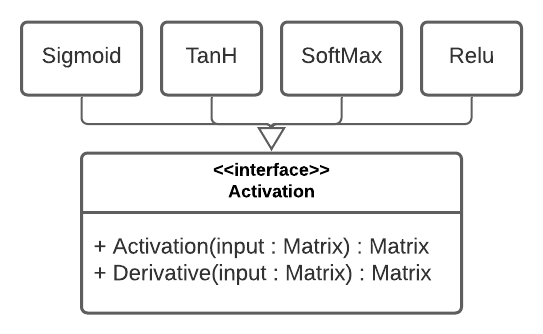
\includegraphics[width=.65\textwidth]{Images/Design/Classes/Activation.png} \\
                    \caption*{The Activation Base Class and Implemented Activations}
                \end{figure}
            \subsubsection{Matrix Class}
                The Matrix Class will contain the standard Matrix Operations, along with multiple methods of creating different 
                Matrices. It is used as an integral part of the NeuralNet Class, because it heavily relies on Matrix Operations.
                These Operations require efficient algorithms, which are outlined under Description of Algorithms. \\
                \vspace{0.2cm}
                This fulfils objectives under \textbf{Objective 3} \\

                \begin{figure}[H]
                    \centering
                    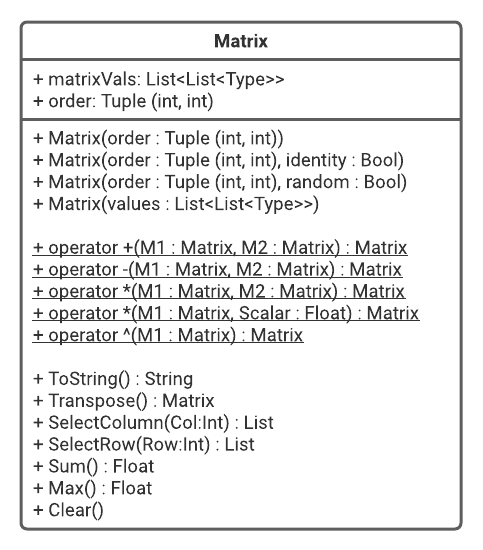
\includegraphics[width=.55\textwidth]{Images/Design/Classes/Matrix.png} \\
                    \caption*{The Matrix Class}
                \end{figure}
            \subsubsection{Deque Class and Experience Replay}
                The Deque Class is used as part of the Implementation of Experience Replay. Within the Deque will be stored instances
                of the Experience Object, which is used to store Individual State Data. The Deque will have Methods to sample states from
                its contents, which will then be used within the DoubleNeuralNet Class to Back Propagate the Calculated Loss.\\
                \vspace{0.2cm}
                This fulfils objectives under \textbf{Objective 5} \\
            
                \begin{figure}[H]
                    \centering
                    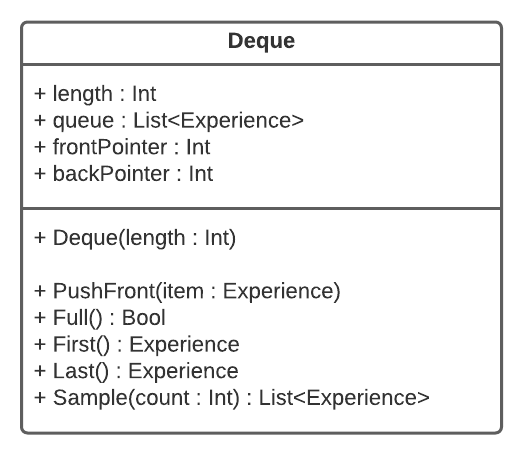
\includegraphics[width=.50\textwidth]{Images/Design/Classes/Deque.png} 
                    \caption*{The Deque Class}
                \end{figure}
                \begin{figure}[H]
                    \centering
                    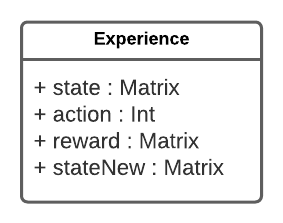
\includegraphics[width=.30\textwidth]{Images/Design/Classes/Experience.png}  \\
                    \caption*{The Experience Class}
                \end{figure}
            \subsubsection{Data Logger and Heap Class}
                The Data Logger Class will be used to Log Data points at certain Points of the Program and then subsequently saving them
                to a .data File. Each Data Point added to the Logger will be checked against the Loggers Structure, which is stored as
                a List of Types. \\
                \vspace{0.2cm}
                These .data files can then be plotted using a Graphing Library. \\
                \vspace{0.2cm}
                This fulfils objectives under \textbf{Objective 8} \\

                \begin{figure}[H]
                    \centering
                    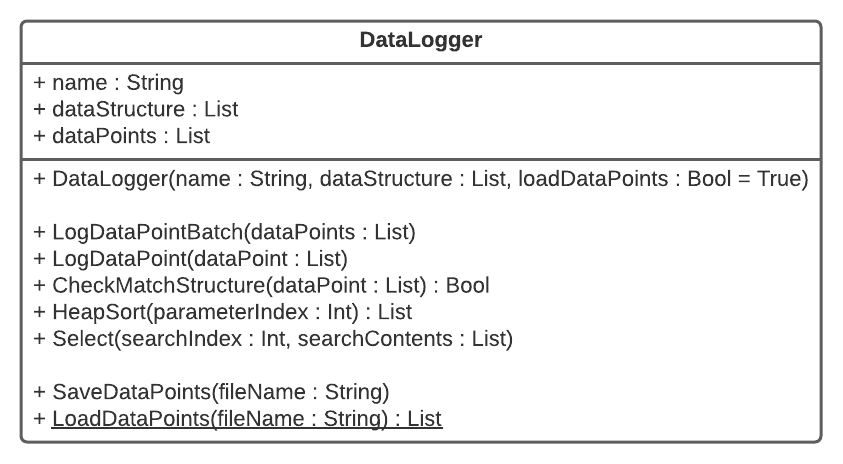
\includegraphics[width=.75\textwidth]{Images/Design/Classes/DataLogger.png}
                    \caption*{The Deque Class}
                \end{figure}
                \begin{figure}[H]
                    \centering
                    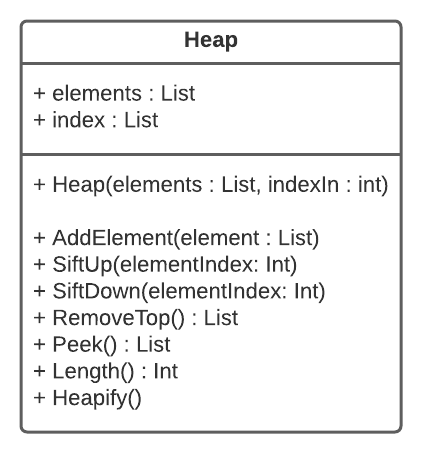
\includegraphics[width=.45\textwidth]{Images/Design/Classes/Heap.png}  \\
                    \caption*{The Experience Class}
                \end{figure}

            \pagebreak
            \vspace{0.5cm}
            \centerline{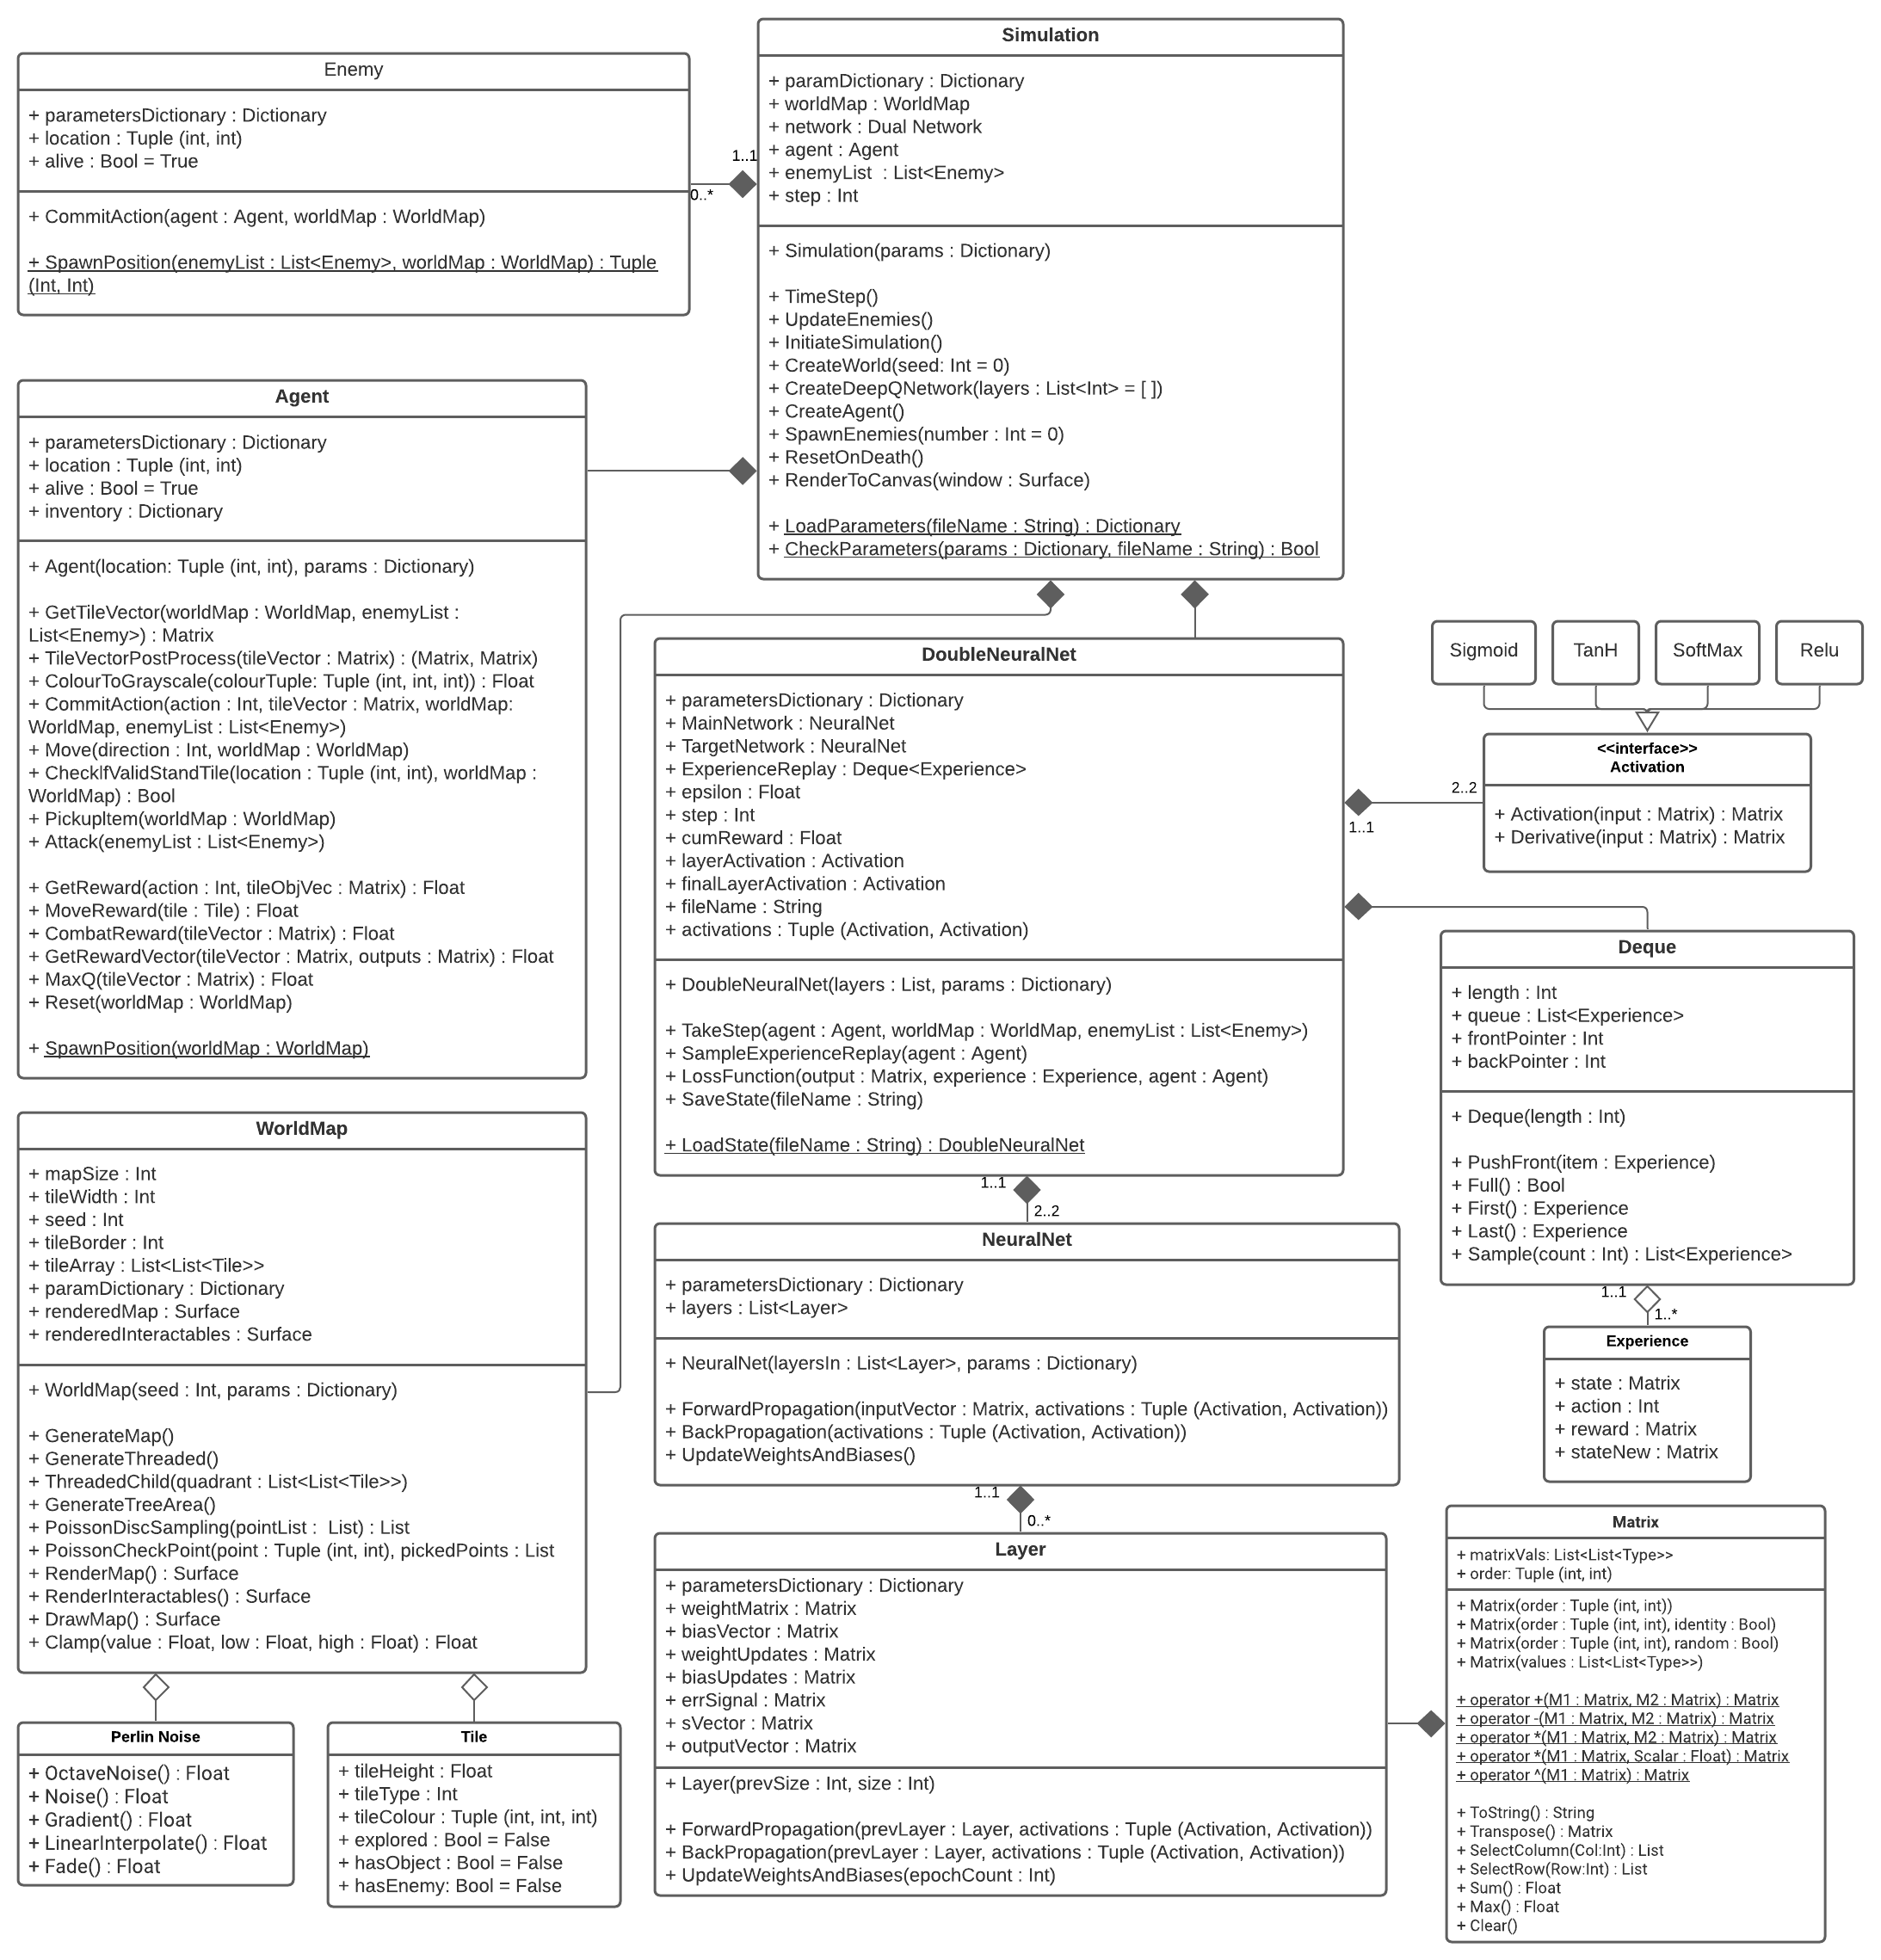
\includegraphics[width=18cm]{Images/Design/ClassDiagram.png}}
            \vspace{0.5cm}
            \pagebreak
        \subsection{Terrain Generation Methods}
            For my Simulation I will need to procedurally generate an Environment. I intend to do this utilising
            the two algorithms, Perlin Noise and Poisson Disc Sampling (as per \textbf{Objective 4.2.2 and 4.2.7}).
            In this section I will explain these two algorithms utilising Diagrams, pseudocode for them can be found under
            the Description of Algorithms Section.

            \subsubsection{Perlin Noise}
                Perlin Noise is a form of Gradient Noise which utilises an initial permutation table of values from $0\to 255$
                to deterministically pick Vectors at each intersection on a Grid. To calculate the Value at a certain point within
                the 2d Grid you calculate each Vector from the corners of the Grid Cell to the specified point. You then
                find the Dot Product between each of these Vectors and the Cells corners. We then use an Interpolation function
                to give us a final value. Below is shown an example of this defined grid with the Vectors attached to each intersection
                point. \\
                \vspace{0.5cm}

                \begin{center}
                    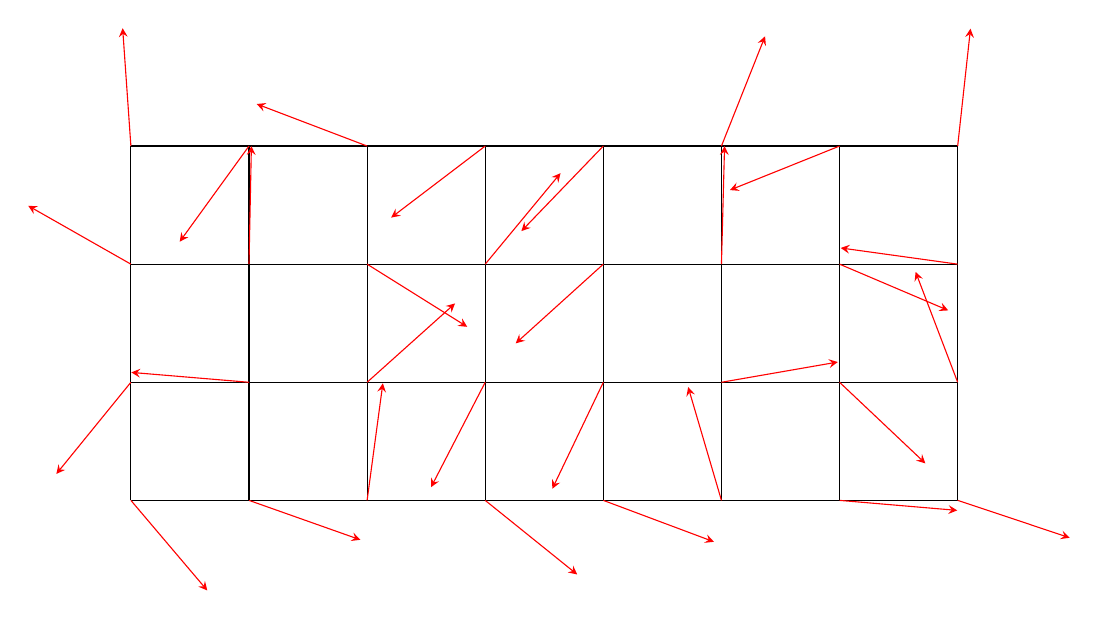
\begin{tikzpicture} [scale=1.5]
                        % Horizontal
                        \draw (-4, 2) -- (3,2);
                        \draw (-4, 1) -- (3,1);
                        \draw (-4, 0) -- (3,0);
                        \draw (-4, -1) -- (3,-1);

                        % Vertical
                        \draw (-4, 2) -- (-4,-1);
                        \draw (-3, 2) -- (-3,-1);
                        \draw (-2, 2) -- (-2,-1);
                        \draw (-1, 2) -- (-1,-1);
                        \draw (0, 2) -- (0,-1);
                        \draw (1, 2) -- (1,-1);
                        \draw (2, 2) -- (2,-1);
                        \draw (3, 2) -- (3,-1);

                        % Vectors
                        \draw [red,-stealth] (-4,-1) -> (-3.3531902939806315,-1.7626514303396656);
                        \draw [red,-stealth] (-4,0) -> (-4.630977086298768,-0.7758014672362491); 
                        \draw [red,-stealth] (-4,1) -> (-4.869274852471338,1.4943290714300883);  
                        \draw [red,-stealth] (-4,2) -> (-4.069776535924549,2.9975626471727828);  
                        \draw [red,-stealth] (-3,-1) -> (-2.057300086127471,-1.3336418324861652);
                        \draw [red,-stealth] (-3,0) -> (-3.996506819243266,0.08351143156280703); 
                        \draw [red,-stealth] (-3,1) -> (-2.9797745644060702,1.9997954449561348); 
                        \draw [red,-stealth] (-3,2) -> (-3.5866712855680216,1.1901748320223897); 
                        \draw [red,-stealth] (-2,-1) -> (-1.8666756238708355,-0.0089275451664651);
                        \draw [red,-stealth] (-2,0) -> (-1.2554466260164219,0.6675629358267805);
                        \draw [red,-stealth] (-2,1) -> (-1.1522871157947239,0.469544661679824);
                        \draw [red,-stealth] (-2,2) -> (-2.934553416957287,2.3558228644332164);
                        \draw [red,-stealth] (-1,-1) -> (-0.22125496971665692,-1.6273405596715351);
                        \draw [red,-stealth] (-1,0) -> (-1.4588750931647785,-0.8885007872101273);
                        \draw [red,-stealth] (-1,1) -> (-0.36250098213671433,1.770451167968059);
                        \draw [red,-stealth] (-1,2) -> (-1.795895289222834,1.3945657024970408);
                        \draw [red,-stealth] (0,-1) -> (0.9364985094954517,-1.350671558174879);
                        \draw [red,-stealth] (0,0) -> (-0.4321341492562097,-0.901809335195978);
                        \draw [red,-stealth] (0,1) -> (-0.7418574353466701,0.32944236219333);
                        \draw [red,-stealth] (0,2) -> (-0.6937822367842611,1.279815157114073);
                        \draw [red,-stealth] (1,-1) -> (0.7181166287846582,-0.04055132235628467);
                        \draw [red,-stealth] (1,0) -> (1.9852224235969194,0.1712798179640916);
                        \draw [red,-stealth] (1,1) -> (1.0263647828314666,1.9996523886963156);
                        \draw [red,-stealth] (1,2) -> (1.369371556758214,2.9292817942142273);
                        \draw [red,-stealth] (2,-1) -> (2.996407526053442,-1.084687909550652);
                        \draw [red,-stealth] (2,0) -> (2.7267142859187103,-0.6869398420834673);
                        \draw [red,-stealth] (2,1) -> (2.9201873668047167,0.6085217630914822);
                        \draw [red,-stealth] (2,2) -> (1.0720411942840524,1.627317219482531);
                        \draw [red,-stealth] (3,-1) -> (3.948643116726071,-1.3163482844717915);
                        \draw [red,-stealth] (3,0) -> (2.6438125421512413,0.9344145198311287);
                        \draw [red,-stealth] (3,1) -> (2.0094614538578335,1.1372347937170555);
                        \draw [red,-stealth] (3,2) -> (3.10861631340332,2.9940837472077853);
                    \end{tikzpicture}
                \end{center}
                
                To sample a specific point on this Grid we need to locate the specific cell that the point
                is contained within. We then find Vectors between each Cells Corners and the Point. The Unit Vectors are
                shown in Red as previous. The Point we are sampling is in Black, pointed to by the newly
                created Green Vectors, which point from the Cell Corners to the Point.

                \begin{center}
                    \begin{tikzpicture} [scale=1.5]
                        % Cell
                        \draw (-1, 1) -> (1, 1);
                        \draw (1, 1) -> (1, -1);
                        \draw (-1, -1) -> (1, -1);
                        \draw (-1, 1) -> (-1, -1);

                        % Unit Vectors
                        \draw [red,-stealth] (-1,-1) -> (-2.7477855439429835,-1.972237467074752);
                        \draw [red,-stealth] (-1,1) -> (-1.7833998754917406,-0.8401860327367792);
                        \draw [red,-stealth] (1,-1) -> (-0.6717240420565347,0.09787919518049071);
                        \draw [red,-stealth] (1,1) -> (2.6385031929005236,2.1468684697273654);

                        % Point
                        \filldraw [black] (-0.2, 0.3) circle (1.5pt);

                        % Vectors
                        \draw [green,-stealth] (-1,-1) -> (-0.2, 0.3);
                        \draw [green,-stealth] (-1,1) -> (-0.2, 0.3);
                        \draw [green,-stealth] (1,-1) -> (-0.2, 0.3);
                        \draw [green,-stealth] (1,1) -> (-0.2, 0.3);
                    \end{tikzpicture}
                \end{center}
            \subsubsection{Poisson Disc Sampling}
                Poisson Disc Sampling is used to create a set of samples, where each sample is between $r$ and $2r$ distance away
                from its Neighbouring Samples. We first define a Grid of Cells with a size r, which allows the Algorithm to shorten the amount of 
                time it takes to determine if a new sample is within the range. A maximum of 1 Sample may be contained within a singular Cell. 
                We then pick a starting point, which can be located anywhere within the Grid. Below is shown an Initial Point, with the Green 
                Hashed Area showing the possible location which the next Sample could lie in. Red is unavailable due to the constraints of the Algorithm.

                \begin{center}
                    \begin{tikzpicture} [scale=1.5]
                        % Horizontal
                        \draw (-3, 1) -- (3,1);
                        \draw (-3, 0) -- (3,0);
                        
                        % Vertical
                        \draw (-2, 2) -- (-2,-1);
                        \draw (-1, 2) -- (-1,-1);
                        \draw (0, 2) -- (0,-1);
                        \draw (1, 2) -- (1,-1);
                        \draw (2, 2) -- (2,-1);

                        \fill [pattern=north east lines, pattern color=green, even odd rule] (0.6, 1.2) circle (.5) circle (1);
                        \fill [pattern=north east lines, pattern color=white] (0, 2) rectangle (1,1);
                        \begin{scope}
                            \clip (0, 2) rectangle (1,1) (0.6, 1.2) circle (.5);
                            \fill [pattern=north east lines, pattern color=red] (0.6, 1.2) circle (1);
                        \end{scope} 

                        \filldraw [green] (0.6, 1.2) circle (1.5pt);
                    \end{tikzpicture}
                \end{center}

                We can then choose a new Sample within this Area. Again is shown the Two areas, Red and Green.

                \begin{center}
                    \begin{tikzpicture} [scale=1.5]
                        % Horizontal
                        \draw (-3, 1) -- (3,1);
                        \draw (-3, 0) -- (3,0);
                        
                        % Vertical
                        \draw (-2, 2) -- (-2,-1);
                        \draw (-1, 2) -- (-1,-1);
                        \draw (0, 2) -- (0,-1);
                        \draw (1, 2) -- (1,-1);
                        \draw (2, 2) -- (2,-1);

                        \fill [pattern=north east lines, pattern color=green, even odd rule] (0.6, 1.2) circle (.5) circle (1);
                        \fill [pattern=north east lines, pattern color=green, even odd rule] (-0.1, 0.8) circle (.5) circle (1);
                        \fill [pattern=north east lines, pattern color=white] (0, 2) rectangle (1,1);
                        \begin{scope}
                            \clip (0, 2) rectangle (1,1) (0.6, 1.2) circle (.5);
                            \fill [pattern=north east lines, pattern color=red] (0.6, 1.2) circle (1);
                        \end{scope} 
                        \fill [pattern=north east lines, pattern color=white] (-1, 1) rectangle (0,0);
                        \fill [pattern=north east lines, pattern color=white] (-0.1, 0.8) circle (.5);
                        \begin{scope}
                            \clip (-1, 1) rectangle (0,0) (-0.1, 0.8) circle (.5);
                            \fill [pattern=north east lines, pattern color=red] (-0.1, 0.8) circle (1.5);
                        \end{scope} 
                        \filldraw [green] (0.6, 1.2) circle (1.5pt);
                        \filldraw [green] (-0.1, 0.8) circle (1.5pt);
                    \end{tikzpicture}
                \end{center}

                This process continues to form a grid of samples. Which my program will use to place items around its
                Environment.
        \subsection{Description of Algorithms}
            \subsubsection{Matrix Addition}
                This algorithm is a Mathematical Operation to add 2 Matrices together. To Add together 2 Matrices their Orders
                must be the same. To perform the Operation you must Sum each element in Matrix A with the corresponding element 
                in Matrix B, placing the result of each Sum in the resultant Matrix.

                \vspace{0.2cm}
                \begin{pseudocode}
|\textbf{SUBROUTINE} MatrixAddition(Matrix1, Matrix2)|
    |TemporaryMatrix \leftarrow \textbf{NEW} Matrix(Matrix1.Order)|
    |\textbf{FOR} Row \leftarrow 0 \textbf{TO} Matrix1.Order[0]|
        |\textbf{FOR} Column \leftarrow 0 \textbf{TO} Matrix1.Order[1]|
            |TemporaryMatrix[Row, Column] \leftarrow Matrix1[Row, Column] + Matrix2[Row, Column]|
        |\textbf{END FOR}|
    |\textbf{END FOR}|
    |\textbf{RETURN} TemporaryMatrix|
|\textbf{ENDSUBROUTINE}|
                \end{pseudocode}

                \vspace{0.5cm}
            \subsubsection{Matrix Subtraction}
                This algorithm is a Mathematical Operation to subtract 2 Matrices. To Subtract 2 Matrices their Orders
                must be the same. To perform the Operation you must Sum each element in Matrix A with the negative of the 
                corresponding element in Matrix B, placing the result of each Sum in the resultant Matrix.

                \vspace{0.2cm}
                \begin{pseudocode}
|\textbf{SUBROUTINE} MatrixSubtraction(Matrix1, Matrix2)|
    |TemporaryMatrix \leftarrow \textbf{NEW} Matrix(Matrix1.Order)|
    |\textbf{FOR} Row \leftarrow 0 \textbf{TO} Matrix1.Order[0]|
        |\textbf{FOR} Column \leftarrow 0 \textbf{TO} Matrix1.Order[1]|
            |TemporaryMatrix[Row, Column] \leftarrow Matrix1[Row, Column] - Matrix2[Row, Column]|
        |\textbf{END FOR}|
    |\textbf{END FOR}|
    |\textbf{RETURN} TemporaryMatrix|
|\textbf{ENDSUBROUTINE}|
                \end{pseudocode}

                \vspace{0.5cm}
            \subsubsection{Matrix Multiplication}
                This algorithm is a Mathematical Operation to find the product of 2 Matrices. To Multiply 2 Matrices
                the number of Columns in the Matrix A must be equal to the number of Rows in Matrix B. Where Matrix A has
                dimensions of $m$ x $n$ and Matrix B has dimensions of $j$ x $k$, the resultant Matrix will have dimensions of 
                $n$ x $j$. To Multiply two Matrices, the algorithm performs the Dot Product between the Row in Matrix A and the 
                corresponding Column in Matrix B. The Dot Product is the Sum of the Products of corresponding elements.

                \vspace{0.2cm}
                \begin{pseudocode}
|\textbf{SUBROUTINE} MatrixMultiplication(Matrix1, Matrix2)|
    |tempMatrix \leftarrow \textbf{NEW} Matrix((Matrix1.Order[0], Matrix2.Order[1]))|
    |\textbf{FOR} i \leftarrow 0 \textbf{TO} Matrix1.Order[0]|
        |\textbf{FOR} j \leftarrow 0 \textbf{TO} Matrix2.Order[1]|
            |\textbf{FOR} l \leftarrow 0 \textbf{TO} Matrix.Order[1]|
                |tempMatrix[i, j] \leftarrow tempMatrix[i, j] + Matrix1[i, k] * Matrix2[k, j]|
            |\textbf{END FOR}|
        |\textbf{END FOR}|
    |\textbf{END FOR}|
    |\textbf{RETURN} tempMatrix|
|\textbf{ENDSUBROUTINE}|
                \end{pseudocode}   

                \vspace{0.5cm}
            \subsubsection{Matrix Scalar Multiplication}
                This algorithm is a Mathematical Operation to find the product between a Matrix and a Scalar.
                The result can be found by Multiplying each element of the Matrix by the Scalar Value to form the Resultant 
                Matrix.

                \vspace{0.2cm}
                \begin{pseudocode}
|\textbf{SUBROUTINE} MatrixScalarMultiplication(Scalar, Matrix)|
    |TemporaryMatrix \leftarrow \textbf{NEW} Matrix(Matrix.Order)|
    |\textbf{FOR} Row \leftarrow 0 \textbf{TO} Matrix.Order[0]|
        |\textbf{FOR} Column \leftarrow 0 \textbf{TO} Matrix.Order[1]|
            |TemporaryMatrix[Row, Column] \leftarrow Scalar * Matrix[Row, Column]|
        |\textbf{END FOR}|
    |\textbf{END FOR}|
    |\textbf{RETURN} TemporaryMatrix|
|\textbf{ENDSUBROUTINE}|
                \end{pseudocode}   
                
                \vspace{0.5cm}
            \subsubsection{Matrix Hadamard Product}
                This algorithm is a Mathematical Operation to another way to find the product between 2 Matrices. Instead of
                applying the Dot Product between Rows and Columns, you find the product between each element in Matrix A
                with the corresponding element in Matrix B, placing the result in the resultant Matrix.

                \vspace{0.2cm}
                \begin{pseudocode}
|\textbf{SUBROUTINE} MatrixHadamardProduct(Matrix1, Matrix2)|
    |TemporaryMatrix \leftarrow \textbf{NEW} Matrix(Matrix1.Order)|
    |\textbf{FOR} Row \leftarrow 0 \textbf{TO} Matrix1.Order[0]|
        |\textbf{FOR} Column \leftarrow 0 \textbf{TO} Matrix1.Order[1]|
            |TemporaryMatrix[Row, Column] \leftarrow Matrix1[Row, Column] * Matrix2[Row, Column]|
        |\textbf{END FOR}|
    |\textbf{END FOR}|
    |\textbf{RETURN} TemporaryMatrix|
|\textbf{ENDSUBROUTINE}|
                \end{pseudocode}   

                \vspace{0.5cm}
            \subsubsection{Matrix Power}
                This algorithm is a Mathematical Operation to find the power of a Matrix. The given Matrix needs to have square dimensions.
                The result can be found by multiplying the given Matrix by itself $n$ amount of times where $n$ is the given power.
                
                \vspace{0.2cm}
                \begin{pseudocode}
|\textbf{SUBROUTINE} MatrixHadamardProduct(Matrix, Power)|
    |TemporaryMatrix \leftarrow \textbf{CLONE} Matrix|
    |\textbf{FOR} Row \leftarrow 0 \textbf{TO} Power - 1|
        |TemporaryMatrix \leftarrow TemporaryMatrix * Matrix|
    |\textbf{END FOR}|
    |\textbf{RETURN} TemporaryMatrix|
|\textbf{ENDSUBROUTINE}|
                \end{pseudocode}  

                \vspace{0.5cm}
            \subsubsection{Matrix Transpose}
                This algorithm is a Mathematical Operation used to Flip a Matrix across its Diagonal. The Transpose of any Matrix
                can be found by converting each Row of the Matrix into a Column. An $m$ x $n$ Matrix will turn into an $n$ x $m$ Matrix.

                \vspace{0.2cm}
                \begin{pseudocode}
|\textbf{SUBROUTINE} MatrixTranspose(Matrix)|
    |TemporaryMatrix \leftarrow \textbf{NEW} Matrix(Matrix.Order)|
    |\textbf{FOR} Row \leftarrow 0 \textbf{TO} Matrix.Order[0]|
        |\textbf{FOR} Column \leftarrow 0 \textbf{TO} Matrix.Order[1]|
            |TemporaryMatrix[Row, Column] \leftarrow Matrix[Column, Row]|
        |\textbf{END FOR}|
    |\textbf{END FOR}|
    |\textbf{RETURN} temporaryMatrix|
|\textbf{ENDSUBROUTINE}|
                \end{pseudocode}

                \vspace{0.5cm}
            \subsubsection{Activation Function SoftMax}
                This algorithm is a logistic function that creates a probability distribution from a set of points. This probability 
                distribution sums to 1. It applies the standard Exponential Function to each element, then normalises this value by dividing
                by the sum of all these Exponentials.

                \vspace{0.2cm}
                \begin{pseudocode}
|\textbf{SUBROUTINE} Softmax(Input)|
    |OutVector \leftarrow \textbf{NEW} Matrix(Input.Order)|
    |ExpSum \leftarrow 0|
    |\textbf{FOR} Row \leftarrow 0 \textbf{TO} Input.Order[0]|
        |ExpSum \leftarrow ExpSum + Math.exp(Input[Row, 0]|)
    |\textbf{END FOR}|
    |\textbf{FOR} Row \leftarrow 0 \textbf{TO} Input.Order[0]|
        |OutVector[Row] \leftarrow Input[Row, 0] / ExpSum|
    |\textbf{END FOR}|
    |\textbf{RETURN} OutVector|
|\textbf{ENDSUBROUTINE}|
                \end{pseudocode}

                \vspace{0.5cm}
            \subsubsection{Neural Network Forward Propagation}
                This algorithm is used to obtain the outputs of a Neural Network. It uses Matrix Multiplication to propagate the inputs
                of the network from Layer to Layer, eventually reaching the Output Layer. My Multiplying the Weight Matrix and the outputs
                of the previous Layer, and then adding the Bias. We can obtain the output of the layer.

                \vspace{0.2cm}
                \begin{pseudocode}
|\textbf{SUBROUTINE} Forward Propagation(PrevLayer, Activations, FinalLayer)|
    |WeightValueProduct \leftarrow This.WeightMatrix * PrevLayer.OutputVector|
    |This.SVector \leftarrow WeightValueProduct + This.BiasVector|
    |\textbf{IF NOT} FinalLayer|
        |This.OutputLayer \leftarrow Activations[0].Activation(SVector)|
    |\textbf{ELSE}|
        |This.OutputLayer \leftarrow Activations[1].Activation(SVector)|
    |\textbf{END IF}| 
|\textbf{ENDSUBROUTINE}|
                \end{pseudocode}

                \vspace{0.5cm}
            \subsubsection{Half Square Difference}  
                This algorithm is the Cost Function of the Neural Network used in tandem with Bellman Equation. It takes the network output
                away from the expected value, squares and then halves it, per output node.

                \begin{pseudocode}
|\textbf{SUBROUTINE} HalfSquareDiff(NetworkOutput, Expected)|  
    |\textbf{RETURN} 0.5 * Math.pow((Expected - NetworkOutput, 2)|
|\textbf{ENDSUBROUTINE}|
                \end{pseudocode}
            \subsubsection{Neural Network Expected Value}
                This algorithm calculates the expected value of the Neural Network. This is calculated using a variation of the Bellman Equation.
                The Bellman Equation is necessary for Mathematically Optimizing in this case. It determines the Value of a decision at a certain 
                point in time, in terms of the Payoff from the Initial Action and the Value of the Potential Payoff after taking that Initial
                Action. 
                
                \vspace{0.2cm}
                \begin{pseudocode}
|\textbf{SUBROUTINE} ExpectedValues(Output, TempExperience, Agent)|  
    |Reward \leftarrow TempExperience.Reward|
    |Gamma \leftarrow LoadFromParameters("DQLGamma")|

    |This.TargetNetwork.ForwardPropagation(TempExperience.State)|
    |TargetNetworkAction \leftarrow This.TargetNetwork.Activations.Max()|
    |NewState \leftarrow Agent.GetNewState(TargetNetworkAction)|
    |TargetRewardMax \leftarrow Agent.GetReward(NewState).Max()|

    |Expected \leftarrow (Reward + (Gamma * TargetRewardMax))|
    |\textbf{RETURN} HadamardProduct(Expected, Expected)|
|\textbf{ENDSUBROUTINE}|
                \end{pseudocode}
                \vspace{0.5cm}
            \subsubsection{Neural Network Backwards Propagation}
                This algorithm is used within a Neural Network to adjust its Weights and Biases, allowing it to more accurately predict the
                best outcome. In Reinforcement Learning, the Network is trained using an estimate for what is the best action given a situation.
                Using this estimate, we can train the Network to predict this outcome by converging the series of Weights and Biases towards a
                local minimum. This is done by calculating partial derivates for every weight and bias value with respect to the cost function.
                This derivative is then subtracted from the existing weight or bias, eventually converging on the best possible value.

                \vspace{0.2cm}
                \begin{pseudocode}
|\textbf{SUBROUTINE} BackPropagation(PreviousLayer, LearningRate, Activation)|
    |WeightTranspose \leftarrow PreviousLayer.WeightMatrix.Transpose()|
    |DeltaWeightProduct \leftarrow WeightTranspose * PreviousLayer.ErrorSignal|
    |This.ErrorSignal \leftarrow DeltaWeightProduct * Activation.Derivative(This.PreActivations)|

    |WeightDerivatives \leftarrow This.ErrorSignal * This.Activations.Transpose()|
    |BiasDerivatives \leftarrow This.ErrorSignal|

    |This.WeightUpdates \leftarrow This.WeightUpdates + (WeightDerivatives * LearningRate)|
    |This.BiasUpdates \leftarrow This.BiasUpdates + (BiasDerivatives * LearningRate)|
|\textbf{ENDSUBROUTINE}|
                \end{pseudocode}

                \vspace{0.5cm}
            \subsubsection{Experience Replay}
                This algorithm samples a Double Ended Queue of (State, Action, Reward, State') Tuples and performs the Back Propagation Algorithm
                on the data. This process is designed to imitate the recall of previous experiences stored in the agents figurative Memory.

                \vspace{0.2cm}
                \begin{pseudocode}
|\textbf{SUBROUTINE} ExperienceReplay(SampleSize, Agent)|
    |Samples \leftarrow \textbf{NEW} List()|
    |\textbf{FOR} i \leftarrow 0 \textbf{TO} SampleSize|
        |Samples.Add(Buffer.RandomSample())|
    |\textbf{END FOR}|

    |\textbf{FOR} Sample \textbf{IN} Samples|
        |PostProcessedSurround \leftarrow Agent.TileVectorPostProcess(sample.state)|

        |NetInput \leftarrow PostProcessedSurround[1]|

        |This.MainNetwork.ForwardPropagation(NetInput, This.Activation)|

        |Output \leftarrow This.MainNetwork.Layers[-1].Activations|

        |ExpectedValues \leftarrow This.ExpectedValue(Output, Sample, Agent)|

        |Cost \leftarrow This.HalfSquareDiff(Output, ExpectedValues)|

        |Preactivations \leftarrow This.MainNetwork.Layers[-1].Preactivations|
        |PreactivationsDerivative \leftarrow This.Activation.Derivative(Preactivations)|
        |This.MainNetwork.Layers.ErrSignal \leftarrow Cost * PreactivationsDerivative|

        |This.MainNetwork.BackPropagation(This.Activation)|
    |\textbf{END FOR}|
|\textbf{ENDSUBROUTINE}|
                \end{pseudocode}

                \vspace{0.5cm}
            \subsubsection{Agent Get Tile Vector}
                This algorithm takes the current World Data of the simulation, and produces a Vector of Tile Data surrounding the Agent. This can
                be done using a nested For Loop rather simply.

                \vspace{0.2cm}
                \begin{pseudocode}
|\textbf{SUBROUTINE} GetTileVector(WorldMap)|
    |Offset \leftarrow LoadFromParameters("DQLOffset")|
    |SideLength \leftarrow 2 * Offset + 1|
    |TileVector \leftarrow \textbf{NEW} Matrix((Math.pow(sideLength, 2), 1))|
    |Num \leftarrow 0|
    |\textbf{FOR} i \leftarrow Agent.Pos[1] - Offset \textbf{TO} Agent.Pos[1] + Offset + 1|
        |\textbf{FOR} j \leftarrow Agent.Pos[0] - Offset \textbf{TO} Agent.Pos[1] + Offset + 1|
            |TileVector[Num, 0] \leftarrow WorldMap[j, i]|
            |Num \leftarrow Num + 1|
        |\textbf{END FOR}|
    |\textbf{END FOR}|
    |\textbf{RETURN} TileVector|
|\textbf{ENDSUBROUTINE}|
                \end{pseudocode}
                
                \vspace{0.5cm}
            \subsubsection{Agent Convert to Greyscale}
                This algorithm converts a given RGB Colour Value to the corresponding Gray Scale Value. The Red, Green and Blue elements of
                the colour value are multiplied by the specific values $0.299$, $0.587$ and $0.114$. You then sum the results, and divide by 
                $255$.

                \vspace{0.2cm}
                \begin{pseudocode}
|\textbf{SUBROUTINE} RGBToGrayscale(RGBVal)|
    |GrayscaleValue \leftarrow 0|
    |GrayscaleValue \leftarrow GrayscaleValue + (0.299 * RGBVal[0])|
    |GrayscaleValue \leftarrow GrayscaleValue + (0.587 * RGBVal[1])|
    |GrayscaleValue \leftarrow GrayscaleValue + (0.114 * RGBVal[2])|
    |\textbf{RETURN} GrayscaleValue / 255|
|\textbf{ENDSUBROUTINE}|
                \end{pseudocode}

                \vspace{0.5cm}
            \subsubsection{Agent Post Process Tile Vector}
                This algorithm will convert the Tile Vector into a Vector of Greyscale values, which can be used as the input for the Neural
                Network.

                \vspace{0.2cm}
                \begin{pseudocode}
|\textbf{SUBROUTINE} GetTileVector(TileVector)|
    |ProcessedVector \leftarrow \textbf{NEW} Matrix(TileVector.Order)|
    |\textbf{FOR} Row \leftarrow 0 \textbf{TO} TileVector.Order[0]|
        |ProcessedVector[Row, 0] \leftarrow RGBToGrayscale(TileVector[Row, 0].RGBValue)|
    |\textbf{END FOR}|
    |\textbf{RETURN} ProcessedVector|
|\textbf{ENDSUBROUTINE}|
                \end{pseudocode}
                
                \vspace{0.5cm}
            \subsubsection{Agent Spawn Position}
                This algorithm will create a list of spawnable tiles for which the Agent could spawn on, and then randomly select a specific
                tile as its spawn position.

                \vspace{0.2cm}
                \begin{pseudocode}
|\textbf{SUBROUTINE} AgentSpawnPosition(WorldMap)|
    |SpawnList \leftarrow \textbf{NEW} List()|
    |MapSize \leftarrow LoadFromParameters("MapSize")|
    |\textbf{FOR} y \leftarrow 0 \textbf{TO} MapSize|
        |\textbf{FOR} x \leftarrow 0 \textbf{TO} MapSize|
            |\textbf{IF} WorldMap[x, y].TileType == 2|
                |SpawnList.Add([x, y])|
            |\textbf{END IF}|
        |\textbf{END FOR}|
    |\textbf{END FOR}|
    |SpawnList.Shuffle()|
    |\textbf{RETURN} SpawnList[0]|
|\textbf{ENDSUBROUTINE}|
                \end{pseudocode}

                \vspace{0.5cm}
            \subsubsection{Enemy Spawn Position}
                This algorithm will create a list of spawnable tiles for which Enemies can spawn on, then select tiles randomly, if they don't
                already contain an enemy or the agent it will create an Enemy Object with that position. It will do this $n$ amount of times 
                where $n$ is the limit to how many enemies can spawn.
                
                \vspace{0.2cm}
                \begin{pseudocode}
|\textbf{SUBROUTINE} EnemySpawnPosition(WorldMap, EnemyList)|
    |SpawnList \leftarrow \textbf{NEW} List()|
    |EnemyLocationList \leftarrow \textbf{NEW} List()|
    |MapSize \leftarrow LoadFromParameters("MapSize")|
    |\textbf{FOR} y \leftarrow 0 \textbf{TO} MapSize|
        |\textbf{FOR} x \leftarrow 0 \textbf{TO} MapSize|
            |\textbf{IF} WorldMap[x, y].TileType == 2|
                |SpawnList.Add([x, y])|
            |\textbf{END IF}|
        |\textbf{END FOR}|
    |\textbf{END FOR}|
    |SpawnList.Shuffle()|
    |\textbf{IF} SpawnList[0] \textbf{IN} EnemyLocationList|
        |\textbf{RETURN NONE}|
    |\textbf{ELSE}|
        |\textbf{RETURN} SpawnList[0]|
    |\textbf{END IF}|
    |\textbf{RETURN} SpawnList[0]|
|\textbf{ENDSUBROUTINE}|
                \end{pseudocode}

                \vspace{0.5cm}
            \subsubsection{Enemy Move}
                The algorithm I have designed for the Enemy Pathfinding is rather simple, and won't take up much runtime in my solution.
                First it calculates the distance between itself and the Agent in both Axis. The Enemy will then converge upon the Agents
                position by moving in the direction with the greatest distance, effectively finding the nearest diagonal and following it.

                \vspace{0.2cm}
                \begin{pseudocode}
|\textbf{SUBROUTINE} EnemyMove(Agent, WorldMap)|
    |XDifference \leftarrow Agent.Pos[0] - This.Pos[0]|
    |YDifference \leftarrow Agent.Pos[1] - This.Pos[0]|

    |\textbf{IF} XDifference == 0 \textbf{AND} YDifference == 0|
        |Agent.Alive = False|
        |\textbf{RETURN}|
    |\textbf{END IF}|

    |\textbf{IF} abs(XDifference) > abs(YDifference)|
        |\textbf{IF} XDifference > 0|
            |This.Pos[0] \leftarrow This.Pos[0] + 1|
        |\textbf{ELSE}|
            |This.Pos[0] \leftarrow This.Pos[0] - 1|
        |\textbf{END IF}|
    |\textbf{ELSE IF} abs(XDifference) < abs(YDifference)|
        |\textbf{IF} YDifference > 0|
            |This.Pos[1] \leftarrow This.Pos[1] + 1|
        |\textbf{ELSE}|
            |This.Pos[1] \leftarrow This.Pos[1] - 1|
        |\textbf{END IF}|
    |\textbf{END IF}|
|\textbf{ENDSUBROUTINE}|
                \end{pseudocode}
                
                \vspace{0.5cm}
            \subsubsection{Poisson Disc Sampling}
                Poisson Disc Sampling is used to sample a set of points in N Dimensional Space. It takes two parameters, $r$ and $k$, where
                $r$ is the minimum distance a specified point must be from every other point, and $k$ is the limit of samples to choose
                before rejection. It starts by creating an N Dimensional Grid which accelerates spacial searches. An initial sample is then
                chosen and inserted into the grid. It then chooses a random point, and determines if it is greater than $r$ range from every 
                other point in the grid. This can easily be accomplished using the previously defined Grid. If after $k$ attempts, no point is
                found then the search is concluded.

                \vspace{0.2cm}
                \begin{pseudocode}
|\textbf{SUBROUTINE} PoissonDiscSampling(PointList)|
    |KVal \leftarrow LoadFromParameters("PoissonKVal")|
    |MapSize \leftarrow LoadFromParameters("MapSize")|
    |PickedPoints \leftarrow \textbf{NEW} Grid(MapSize, MapSize)|
    |SampleNum \leftarrow LoadFromParameters("MapSize")|
    |\textbf{WHILE} SampleNum <= KVal|
        |Sample \leftarrow PointList[RandomInt(0, PointList.Length - 1)]|
        |Result \leftarrow CheckPointDistance(Sample, PickedPoints)|
        |\textbf{IF} Result == True|
            |PickedPoints[Sample[0], Sample[1]] \leftarrow True|
            |SampleNum \leftarrow 0|
            |\textbf{CONTINUE}|
        |\textbf{ELSE}|
            |SampleNum \leftarrow SampleNum + 1|
            |\textbf{CONTINUE}|
        |\textbf{END IF}|
    |\textbf{END WHILE}|
    |\textbf{RETURN} PickedPoints|
|\textbf{ENDSUBROUTINE}|
                \end{pseudocode}
                
                \vspace{0.5cm}
            \subsubsection{Perlin Noise}
                Perlin Noise is a method of generating a procedural texture depending upon input parameters. It defines an n-dimensional
                grid of Vectors, each grid intersection contains a fixed, random unit vector. To sample Perlin Noise, the grid cell which
                the point lies in must be found. The Vectors between the sampled point, and the corners of the cell. We then take the Dot
                Product between these new Vectors, and the Vectors applied to the intersections. In 2d Space this leaves us with 4 Values.
                We then use an Interpolation function to Interpolate between the 4 Values. 
            
                \vspace{0.2cm}
                \begin{pseudocode}
|PermTable \leftarrow [1 \rightarrow 255].Shuffle() * 2|

|\textbf{SUBROUTINE} PerlinNoise(X, Y)|
    |XFloor \leftarrow Math.floor(X)|
    |YFloor \leftarrow Math.floor(Y)|

    |G1 \leftarrow PermTable[PermTable[XFloor] + YFloor]|
    |G2 \leftarrow PermTable[PermTable[XFloor + 1] + YFloor]|
    |G3 \leftarrow PermTable[PermTable[XFloor] + YFloor + 1]|
    |G4 \leftarrow PermTable[PermTable[XFloor + 1] + YFloor + 1]|

    |XExact \leftarrow X - XFloor|
    |YExact \leftarrow Y - YFloor|

    |D1 \leftarrow Grad(G1, XFloor, YFloor)|
    |D2 \leftarrow Grad(G2, XFloor - 1, YFloor)|
    |D3 \leftarrow Grad(G3, XFloor, YFloor - 1)|
    |D4 \leftarrow Grad(G4, XFloor - 1, YFloor - 1)|

    |U \leftarrow Fade(XFloor)|
    |V \leftarrow Fade(YFloor)|

    |XInterpolated \leftarrow Lerp(U, D1, D2)|
    |YInterpolated \leftarrow Lerp(U, D3, D4)|

    |\textbf{RETURN} Lerp(V, XInterpolated, YInterpolated)|
|\textbf{ENDSUBROUTINE}|

|\textbf{SUBROUTINE} Grad(Hash, X, Y)|
    |Temp \leftarrow Hash BITWISEAND 3|
    |\textbf{IF} Temp == 0|
        |\textbf{RETURN} X + Y|
    |\textbf{ELSE IF} Temp == 1|
        |\textbf{RETURN} -X + Y|
    |\textbf{ELSE IF} Temp == 2|
        |\textbf{RETURN} X - Y|
    |\textbf{ELSE IF} Temp == 3|
        |\textbf{RETURN} -X - Y|
    |\textbf{ELSE}|
        |\textbf{RETURN} 0|
    |\textbf{END IF}|
|\textbf{ENDSUBROUTINE}|

|\textbf{SUBROUTINE} Lerp(Ammount, Left, Right)|
    |\textbf{RETURN} ((1 - Ammount) * Left + Ammount * Right)|
|\textbf{ENDSUBROUTINE}|

|\textbf{SUBROUTINE} Fade(T)|
    |\textbf{RETURN} T * T * T * (T * (T * 6 - 15) + 10)|
|\textbf{ENDSUBROUTINE}|
                \end{pseudocode}

                \vspace{0.5cm}
            \subsubsection{Octave Perlin Noise}
                Octave Perlin Noise takes the existing Perlin Noise algorithm, but adds rescaled clones of itself into itself, to create
                what is known as Fractal Noise. Creating this Fractal Noise is common practice because it reduces the sharp edges encountered
                with just the regular Perlin Noise Algorithm.

                \vspace{0.2cm}
                \begin{pseudocode}
|\textbf{SUBROUTINE} OctaveNoise(X, Y, Octaves, Persistence)|
    |Total \leftarrow 0|
    |Frequency \leftarrow 1|
    |Amplitude \leftarrow 1|
    |MaxValue \leftarrow 0|

    |\textbf{FOR} i \leftarrow 0 \textbf{TO} Octaves|
        |Total \leftarrow Total + (PerlinNoise(X * Frequency, Y * Frequency) * Amplitude|

        |MaxValue \leftarrow MaxValue + Amplitude|

        |Amplitude \leftarrow Amplitude * Persistence|
        |Frequency \leftarrow Frequency * 2|
    |\textbf{END FOR}|

    |\textbf{RETURN} Total / MaxValue|
|\textbf{ENDSUBROUTINE}|            
                \end{pseudocode}
            \subsubsection{Heap Heapify}
                The Heapify algorithm converts a Binary Tree of values into a valid Heap. A Diagram for this process, along with the Heap Property is shown when descibing the Heap 
                Data Structure under Description of Data Structures. This algorithm works by repeatedly performing Sift Down Operations for \textbf{$\lfloor$(N-1)/2$\rfloor$} times.
                Where N is the Number of elements in the Tree. A Sift Down Operation will swap elements which don't conform to the Heap Property.
                This operation relies on the fact that Children of an Index are located at \textbf{2i + 1} and \textbf{2i + 2}.
                \vspace{0.2cm}

                \begin{pseudocode} 
|\textbf{SUBROUTINE} Heapify()|
    |\textbf{FOR} i \leftarrow $\lfloor$(HeapList.Length-1)/2$\rfloor$ \textbf{TO} 0 \textbf{STEP} -1|
        |SiftDown(i)|
    |\textbf{END FOR}|
|\textbf{ENDSUBROUTINE}| 

|\textbf{SUBROUTINE} SiftDown(RootIndex)|
    |IsHeap \leftarrow \textbf{FALSE}|
    |End \leftarrow HeapList.Length - 1|

    |\textbf{WHILE} (2 * RootIndex) + 1 <= End|
        |ChildIndex = (RootIndex * 2) + 1|
        |\textbf{IF} ChildIndex <= End \textbf{AND} HeapList[ChildIndex] < HeapList[ChildIndex + 1]|
            |ChildIndex \leftarrow ChildIndex + 1|
        |\textbf{END IF}|
        |\textbf{IF} HeapList[RootIndex] < HeapList[ChildIndex]|
            |TempSwap \leftarrow HeapList[ChildIndex]|
            |HeapList[ChildIndex] \leftarrow HeapList[RootIndex]|
            |HeapList[RootIndex] \leftarrow TempSwap|
        |\textbf{ELSE}|   
            |\textbf{BREAK}|
        |\textbf{END IF}|
|\textbf{ENDSUBROUTINE}| 
                \end{pseudocode}

                \vspace{0.5cm}
            \subsubsection{Heap Extraction}
                This algorithm extracts the Root Element from a valid Heap. It does this by swapping the Root Element and Final Element, and then
                popping the new Final Element (Originally the Root) from the list. 
                \vspace{0.2cm}

                \begin{pseudocode}
|\textbf{SUBROUTINE} RemoveTop()|
    |TempSwap \leftarrow HeapList[-1]|
    |HeapList[-1] \leftarrow HeapList[0]|
    |HeapList[0] \leftarrow TempSwap|
    |ReturnItem \leftarrow HeapList.Pop()|

    |Heapify()|

    |\textbf{RETURN} ReturnItem|
|\textbf{ENDSUBROUTINE}| 
                \end{pseudocode}

                \vspace{0.5cm}
            \subsubsection{Heap Sort}
                The Heap Sort algorithm relies on the prior two algorithms to fully order a list in Worst and Best case $O(nlog(n))$ Time Complexity. It 
                is also $O(1)$ Space Complexity due to it being an In-Place Sorting algorithm. The sort will iteratively shrink the unsorted region by 
                performing the following steps: Apply Heapify to the Unsorted Region, Extract the Root Element from the Heap, Insert the Extracted Element 
                at the end of the Unsorted Region. This allows it to be In-Place because it never requires extra space.
                \vspace{0.2cm}

                \begin{pseudocode}
|\textbf{SUBROUTINE} HeapSort()|
    |SortedList \leftarrow \textbf{NEW} List()|
    |Heap \leftarrow \textbf{NEW} Heap(DataPoints)|

    |\textbf{WHILE} Heap.Size() - 1 >= 0|
        |SortedList.Append(Heap.RemoveTop)|
    |\textbf{END FOR}|

    |\textbf{RETURN} SortedList|
|\textbf{ENDSUBROUTINE}|
                \end{pseudocode}

                \vspace{0.5cm}
            \subsubsection{Deque Push Front}
                This Algorithm pushes an item to the front of a Double Ended Queue. If an Item exists in the new position, it will be overwritten by
                the new Item. A Diagram for this process is shown when describing the Deque Data Structure under Description of Data Structures.
                \vspace{0.2cm}

                \begin{pseudocode}
|\textbf{SUBROUTINE} PushFront(Item)|
    |This.FrontPointer \leftarrow (This.FrontPointer + 1) % This.Length|

    |\textbf{IF} This.IsFull()|
        |This.BackPointer = (This.FrontPointer + 1) % This.Length|
    |\textbf{END IF}|
    
    |This.Queue[This.FrontPointer] = Item|
|\textbf{ENDSUBROUTINE}|
                \end{pseudocode}

                \vspace{0.5cm}
            \subsubsection{Deque Full}
                This simple Algorithm Determines if a Double Ended Queue is Full or Not. It simply checks if the next position in front of the
                Front Pointer is free or not.
                \vspace{0.2cm}

                \begin{pseudocode}
|\textbf{SUBROUTINE} IsFull()|
    |\textbf{IF} This.Queue[(This.FrontPointer + 1) % This.Length] != None|
        |\textbf{RETURN} \textbf{TRUE}|
    |\textbf{END IF}|
    |\textbf{RETURN} \textbf{FALSE}|
|\textbf{ENDSUBROUTINE}|
                \end{pseudocode}

                \vspace{0.5cm}
        \subsection{Description of Data Structures}
            \subsubsection{Matrices}
                A Matrix is a rectangular array of numbers which can be used in arithmetic operations such as Addition and Multiplication.
                They are essentially a 2d Array of Values, as shown below. \\
                \begin{center}
                    $\begin{bmatrix}
                        a & b\\
                        c & d
                    \end{bmatrix}$ 
                    $\begin{bmatrix}
                        a & b & c \\
                        d & e & f \\
                        g & h & i 
                    \end{bmatrix}$ 
                    $\begin{bmatrix}
                        a \\
                        b \\
                        c  
                    \end{bmatrix}$ 
                    $\begin{bmatrix}
                        a & b & c & d\\
                        e & f & g & h
                    \end{bmatrix}$ 
                \end{center}    
                They are commonly used within Computer Science due to their efficient implementations, this is specifically helpful
                within the field of Machine Learning due to being able to store the various elements of a Neural Network within Matrices.
                This allows us to perform Matrix Operations between these elements in order to speed up the Forward and Back Propagation 
                Process. \\
                \vspace{0.2cm}
                In my Program Matrices will be able to be defined by multiple different Methods. Such as a Tuple of Integers, existing 2d
                List or existing 1d List (as per \textbf{Objective 3.3}). This will allow Matrices to be created easily and efficiently
                within the Program, without having to populate them with values manually. Matrices will also be able to populated automatically
                with random values (as per \textbf{Objective 3.4}), this will be used when generating untrained Weights and Biases for the 
                Neural Network implementation. \\
                \vspace{0.2cm}
                When using Matrices as part of Arithmetic Operations, the use of Operator Overloading for the Standard Operations will be
                useful to make Code Cleaner and more Readable (as per \textbf{Objective 3.8}).
            \subsubsection{Double Ended Queue} 
                A Double Ended Queue (Commonly referred to as a Deque) is an Abstract Data Type, which is a generalization of 
                a Queue. Elements can be added to the Front/Head or Back/Tail. Deques are commonly implemented using an Array, and two
                pointers, one for Front and Back. The Deque in my program will be utilised within the Experience Replay Algorithm (as per 
                \textbf{Objective 5.12})\\
                \vspace{0.2cm}
                Below is shown an example of a Double Ended Queue:\\ 
                \vspace{1cm}

                \begin{center}
                    \begin{tabular}{ C{1cm} C{1cm} C{1cm} C{1cm} C{1cm} C{1cm} }
                        & \centerline{Back Pointer} &  &  & \centerline{Front Pointer} & \\ 
                        \rule{0pt}{1.2cm}% %
                         & {\Huge $\Downarrow$} &  &  & {\Huge $\Downarrow$} & \\ 
                        \hline
                        \multicolumn{1}{|C{1cm}|}{} & \multicolumn{1}{C{1cm}|}{3} & \multicolumn{1}{C{1cm}|}{6} & \multicolumn{1}{C{1cm}|}{4} & \multicolumn{1}{C{1cm}|}{2} & \multicolumn{1}{C{1cm}|}{} \\ \hline
                    \end{tabular}
                \end{center}

                The Elements are stored within the Array, with the Front and Back Pointer determining the Range of the actual contained Items.
                We can Pop/Remove elements from both the Front and Back of the Queue, or Push them. This can be done by incrementing the pointers
                and overwriting the existing elements should they exist.
                \begin{center}
                    \begin{tabular}{ C{1cm} C{1cm} C{1cm} C{1cm} C{1cm} C{1cm} }
                        & Front & Back &  &  & \\ 
                        \rule{0pt}{1.2cm}% %
                         & {\Huge $\Downarrow$} & {\Huge $\Downarrow$} & & & \\ 
                        \hline
                        \multicolumn{1}{|C{1cm}|}{9} & \multicolumn{1}{C{1cm}|}{3} & \multicolumn{1}{C{1cm}|}{6} & \multicolumn{1}{C{1cm}|}{4} & \multicolumn{1}{C{1cm}|}{2} & \multicolumn{1}{C{1cm}|}{8} \\ \hline
                    \end{tabular} \\
                    \vspace{1cm}
                    When Push the Item $10$ to the Deque: \\
                    \begin{tabular}{ C{1cm} C{1cm} C{1cm} C{1cm} C{1cm} C{1cm} }
                         & & Front & Back &  & \\ 
                        \rule{0pt}{1.2cm}% %
                         & & {\Huge $\Downarrow$} & {\Huge $\Downarrow$} & & \\ 
                        \hline
                        \multicolumn{1}{|C{1cm}|}{9} & \multicolumn{1}{C{1cm}|}{3} & \multicolumn{1}{C{1cm}|}{10} & \multicolumn{1}{C{1cm}|}{4} & \multicolumn{1}{C{1cm}|}{2} & \multicolumn{1}{C{1cm}|}{8} \\ \hline
                    \end{tabular}
                \end{center}             
            \subsubsection{Tile} 
                A Tile is used to store specific location Data as part of the World Map (as per \textbf{Objective 4.2.3}). It can be initialised without values, and is
                then populated with the relevant information. Methods are attatched to this Class to Add/Remove Items and Enemies as needed.
                Allowing for the Agent when getting Tile data to get relevant and accurate information.
            \subsubsection{Experience} 
                An Experience is used to store data for Experience Replay (as per \textbf{Objective 5.9}). It is an Empty Class with no Methods. This includes the State, 
                Action, NewState and Reward, all at the time of assignment. This is used in conjunction with the Experience Replay 
                Algorithm, described above.
            \subsubsection{Heap} 
                A Heap is specialised Binary Tree which satisfies the Heap Property: such that for all nodes with Parents, the
                Parent has a greater value than the Child. A Heap is used as part of a Heap Sort (as per \textbf{Objective 7.5}), an $O(nlog(n))$ Sorting Algorithm. The
                highest priority element is always stored at the Root, with the tree of the structure being considered "Partialy Ordered".
                Heaps can be stored in an Array, with the Root element at Index 0. Children of an Index are located at \textbf{2i + 1} and
                \textbf{2i + 2}. The Parent of an Index is located at \textbf{$\lfloor$(i-1)/2$\rfloor$}. Below is shown an example of items
                stored in a Heap.

                \begin{figure}[H]
                    \centering
                    \subfloat
                    {
                      \begin{tikzpicture}
                        [
                        sibling distance        = 5em,
                        level distance          = 5em,
                        edge from parent/.style = {draw, -latex},
                        every node/.style       = {font=\huge},
                        level 1/.style={sibling distance=8em},
                        level 2/.style={sibling distance=4em},
                        sloped
                        ]
                        \node [badtreenode] {5}
                        child {node [treenode] {7}
                          child {node [treenode] {4}}
                          child {node [treenode] {2}}}
                        child {node [badtreenode] {8}
                          child {node [treenode] {3}}
                          child[fill=none] {edge from parent[draw=none]}};
                      \end{tikzpicture}
                    }
                \end{figure}

                But this Binary Tree violates the Heap Property, because 5 is at the Root of the Tree. 8 is Greater than 5
                so in this case we need to swap these two Items. Once swapped, the actual Heap will look like what is shown below.
                This is then a valid

                \begin{figure}[H]
                    \centering
                    \subfloat
                    {
                      \begin{tikzpicture}
                        [
                        sibling distance        = 5em,
                        level distance          = 5em,
                        edge from parent/.style = {draw, -latex},
                        every node/.style       = {font=\huge},
                        level 1/.style={sibling distance=8em},
                        level 2/.style={sibling distance=4em},
                        sloped
                        ]
                        \node [selectedtreenode] {8}
                        child {node [treenode] {7}
                          child {node [treenode] {4}}
                          child {node [treenode] {2}}}
                        child {node [selectedtreenode] {5}
                          child {node [treenode] {3}}
                          child[fill=none] {edge from parent[draw=none]}};
                      \end{tikzpicture}
                    }
                \end{figure}

                If we were to add a new item to this Heap, it would be appended to the end of the Heaps internal 
                storage Array, and then Sifted up through the Heap. This process can be seen below.

                \begin{figure}[H]
                    \centering
                    \subfloat
                    {
                      \begin{tikzpicture}
                        [
                        sibling distance        = 5em,
                        level distance          = 5em,
                        edge from parent/.style = {draw, -latex},
                        every node/.style       = {font=\huge},
                        level 1/.style={sibling distance=8em},
                        level 2/.style={sibling distance=4em},
                        sloped
                        ]
                        \node [treenode] {8}
                        child {node [treenode] {7}
                          child {node [treenode] {4}}
                          child {node [treenode] {2}}}
                        child {node [badtreenode] {5}
                          child {node [treenode] {3}}
                          child {node [badtreenode] {9}}};
                      \end{tikzpicture}
                    }
                \end{figure}
                \begin{figure}[H]
                    \centering
                    \subfloat
                    {
                      \begin{tikzpicture}
                        [
                        sibling distance        = 5em,
                        level distance          = 5em,
                        edge from parent/.style = {draw, -latex},
                        every node/.style       = {font=\huge},
                        level 1/.style={sibling distance=8em},
                        level 2/.style={sibling distance=4em},
                        sloped
                        ]
                        \node [badtreenode] {8}
                        child {node [treenode] {7}
                          child {node [treenode] {4}}
                          child {node [treenode] {2}}}
                        child {node [badtreenode] {9}
                          child {node [treenode] {3}}
                          child {node [selectedtreenode] {5}}};
                      \end{tikzpicture}
                    }
                \end{figure}
                \begin{figure}[H]
                    \centering
                    \subfloat
                    {
                      \begin{tikzpicture}
                        [
                        sibling distance        = 5em,
                        level distance          = 5em,
                        edge from parent/.style = {draw, -latex},
                        every node/.style       = {font=\huge},
                        level 1/.style={sibling distance=8em},
                        level 2/.style={sibling distance=4em},
                        sloped
                        ]
                        \node [selectedtreenode] {9}
                        child {node [treenode] {7}
                          child {node [treenode] {4}}
                          child {node [treenode] {2}}}
                        child {node [selectedtreenode] {8}
                          child {node [treenode] {3}}
                          child {node [treenode] {5}}};
                      \end{tikzpicture}
                    }
                \end{figure}
        \subsection{File Structure}
            \subsubsection{User Defined Parameters}
                As part of my Technical Solution, the User will be able to modify the parameters which dynamically modifies the Simulation
                and the Structure of the Double Neural Network. The file is stored in a JSON format (Java Script Object Notation).
                This allows the File to be Human Readable, and easily editable. Each parameter will also have a defined Range alongside it.
                The program will throw an error if the parameter is outside the specified range. Below is a table of the Parameters used in
                the Technical Solution, alongside their respective Ranges. \\

                \vspace{0.5cm}

                \normalsize
                \begin{longtable}{| C{4cm} | C{2cm} | C{1.5cm} | C{8cm} |}
                    \hline
                    Name in JSON & Data Type & Range & Description \\
                    \hline\hline
                    EnterValues & Int & 0 - 1 & The program will ask you to enter values if this is 1 \\
                    \hline
                    GenerateThreaded & Int & 0 - 1 & The program will generate the Terrain using Multiple Threads \\
                    \hline
                    EnableEnemies & Int & 0 - 1 & Toggled Enable Enemies Option. \\
                    \hline
                    SaveWeights & Int & 0 - 1 & Toggled Save Network Weights Option. \\
                    \hline
                    StepDelay & Float & 0 - \infty & The time delay each step. \\
                    \hline
                    Debug & Int & 0 - 1 & Toggled Debug Option. \\
                    \hline
                    DebugScale & Int & 1 - 4 & The scale of the Debug side extension. \\
                    \hline
                    WorldSize & Int & 16 - 1024 & The size the of the World in Tiles. Must be a Multiple of 2. \\
                    \hline
                    TileWidth & Int & 1 - 8 & The Width and Height of each Tile. \\
                    \hline
                    TileBorder & Int & 0 - 3 & The Pixel Border surrounding Tiles. \\
                    \hline
                    OctavesTerrain & Int & 1 - 20 & The Perlin Noise Octave Value for World Generation. \\
                    \hline
                    PersistenceTerrain & Float & 0 - 1 & The Perlin Noise Persistence Value for World Generation. \\
                    \hline
                    WorldScale & Float & 0.1 - 10 & The Perlin Noise Scale Value for World Generation. \\
                    \hline
                    OctavesTrees & Int & 1 - 20 & The Perlin Noise Octave Value for Trees \\
                    \hline
                    PersistenceTrees & Float & 0 - 1 & The Perlin Noise Persistence Value for generating the Trees. \\
                    \hline
                    PoissonKVal & Int & 0 - \infty & The K Value for Poisson Disc Sampling. \\
                    \hline
                    TreeSeedOffset & Int & 0 - \infty & The Seed offset for generating the Trees. \\
                    \hline
                    TreeHeight & Float & 0 - 1 & The difference between Min Tree spawning height and Max Tree spawning height. \\
                    \hline
                    InteractableTileBorder & Int & 0 - 3 & The Pixel Border surrounding Interactables. \\
                    \hline
                    TreeBeachOffset & Float & 0 - 1 & The height difference from Beaches which Trees will Spawn. \\
                    \hline
                    Grayscale & Int & 0 - 1 & Toggled Grayscale Terrain Option. \\
                    \hline
                    Water & Float & 0 - 1 & The cuttoff values for Water. \\
                    \hline
                    Coast & Float & 0 - 1 & The cuttoff values for Coast. \\
                    \hline
                    Grass & Float & 0 - 1 & The cuttoff values for Grass. \\
                    \hline
                    Mountain & Float & 0 - 1 & The cuttoff values for Mountains. \\
                    \hline
                    TreeType & String & - & The internally used Inventory name for collected Trees. \\
                    \hline
                    StartEnemyCount & Int & 0 - \infty & The maximum count of Enemies to Spawn upon the creation of a new Map. \\
                    \hline
                    ColourWater & [Int, Int, Int] & 0 - 255 & The display Colour of Water. \\
                    \hline
                    ColourCoast & [Int, Int, Int] & 0 - 255 & The display Colour of Coast. \\
                    \hline
                    ColourGrass & [Int, Int, Int] & 0 - 255 & The display Colour of Grass. \\
                    \hline
                    ColourMountain & [Int, Int, Int] & 0 - 255 & The display Colour of Mountains. \\
                    \hline
                    ColourTree & [Int, Int, Int] & 0 - 255 & The display Colour of Trees. \\
                    \hline
                    ColourPlayer & [Int, Int, Int] & 0 - 255 & The display Colour of the Agent. \\
                    \hline
                    ColourEnemy & [Int, Int, Int] & 0 - 255 & The display Colour of Enemies. \\
                    \hline
                    MoveReward & Float & -1 - 1 & The Reward Gained when the Agent Moves. \\
                    \hline
                    CollectItemReward & Float & -1 - 1 & The Reward Gained when the Agent collects an Item. \\
                    \hline
                    DeathReward & Float & -1 - 1 & The Reward Gained when the Agent Dies through any means. \\
                    \hline
                    ExploreReward & Float & -1 - 1 & The Reward Gained when the Agent moves into a Tile which hasnt been Visited yet. \\
                    \hline
                    AttackReward & Float & -1 - 1 & The Reward Gained when the Agent successfully Attacks an Enemy. \\
                    \hline
                    AttackFailedReward & Float & -1 - 1 & The Reward Gained when the Null Action is chosen. \\
                    \hline
                    NoopReward & Float & -1 - 1 & The Reward Gained when the Null Action is chosen. \\
                    \hline
                    TargetReplaceRate & Int & 5 - 300 & Replace Rate for Target Neural Network. \\
                    \hline
                    EREnabled & Int & 0 - 1 & Wether Experience Replay is Enabled or Disabled. \\
                    \hline
                    ERBuffer & Int & 1k - 10k & The size of the Experience Replay Buffer. \\
                    \hline
                    ERSampleRate & Int & 1 - 100 & The ammount of steps between each Experience Replay sample. \\
                    \hline
                    ERSampleSize & Int & 10 - 1000 & The ammount of samples taken from the Experience Replay Buffer. \\
                    \hline
                    DeepQLearningLayers & [Int, ..., Int] & 0 - 256 & List of Integers defining the size of each Layer in the Neural Network. \\
                    \hline
                    DQLEpoch & Int & 10 - 1000 & The ammount of steps per Weight and Bias Update, along with Network Saving and Debug Output \\
                    \hline
                    DQLearningMaxSteps & Int & 1000 - \infty & Maximum steps the Simulation will run for. \\
                    \hline
                    DQLOffset & Int & 1 - 10 & The square radius around the agent which is sampled for the Input vector, must be the root of the 
                    Input Layers size. \\
                    \hline
                    DQLEpsilon & Float & 0 - 1 & The initial Probability that the Agent will favour a Random Action over the predicted Action \\
                    \hline
                    DQLEpsilonRegression & Float & 0 - 1 & The rate at which Epsilon will decrease, Epsilon is multiplied every step by this number \\
                    \hline
                    DQLLearningRate & Float & 0 - 1 & The Learning Rate of the Neural Network. Higher values will cause more drastic changes during
                    Back Propagation. \\
                    \hline
                    DQLGamma & Float & 0 - 1 & The Discount for future gained Reward \\
                    \hline
                \end{longtable}
            \subsubsection{.dqn Files}
                DQN Files are used to store all Data relating to the Dual Neural Network. It is a Binary File. It contains all Layer Data, along
                with Experience Replay Data, the activations being used, and other important data.
            \subsubsection{.data Files}
                Data Files are used to store all data points created by the Data Loggers. They are Binary Files and are individually created per Data
                Logger.
        \subsection{Integrity and Exception Handling}
            \subsubsection{Ranges}
                As mentioned above under File Structure, I have implemented a Range JSON File, in order to specify the ranges of each parameter the User can
                input. This is used to help the user avoid breaking the simulation by creating unintended results. Things such as creating a very large Neural
                Network would take up alot of memory, possibly causing Memory Allocation issues with the Users system. There is no need to implement Exceptions 
                for most sections of the Project due to the Nature of the system being Dynamically created by the users Json Input. Which is of course sanitised 
                by the Range File.
            \subsubsection{Data Logger Structure Matching}   
                As part of my Data Logger I will implement a system to check if a New Data Point Matches the structure of the Data Logger. This structure will
                be stored as a List of Types, such as [[Int, Float], String, Int], where a nested list represents a multi-typing scenario. This multi-typing 
                scenario would be cases like [Int, Float] where they are interchangeable in some cases. If a New Data Point does not match the structure of
                the Data Logger it will throw an appropriate error.
            \subsubsection{Matrix Exceptions}    
                As part of my Matrix Class I made a series of appropriate Exceptions to help while developing and implementing any Matrix related Logic. These
                Exceptions are thrown when any misintended methods or operations are performed. Such as Multiplying incompatably Matrices, or utilising a non-existant
                initialisation case. Below is shown a Table of Exceptions I have made:

                \begin{center}
                    \begin{tabular}{| L{5cm} | L{10cm} |}
                        \hline
                        Exception Identifier & Exception Message \\
                        \hline
                        \hline
                        NoMatchingInitCase & No Matching Init case for given parameters \\
                        \hline
                        UnableToCreateIdentityMat & Unable to create identity Matrix from given arguments \\
                        \hline
                        NotOfTypeVector & Given list of Vectors contains a Matrix \\
                        \hline
                        VectorsNotOfSameLength & All Vectors must be the same height \\
                        \hline
                        NoMatchingMultiplycase & No matching multiply case found \\
                        \hline
                        NoMatchingAdditionCase & No matching addition case found \\
                        \hline
                        NoMatchingSubtractionCase & No matching addition case found \\
                        \hline
                        NoMatchingPowerCase & No matching power case was found \\
                        \hline
                        MismatchOrders & Orders of Matrices do not match \\
                        \hline
                        SumOfMatrixReqNumericalVals & The sum of a Matrix requires Numerical values \\
                        \hline
                        ColumnOutOfRange & Specified Column out of range of Matrix \\
                        \hline
                        ColumnMustBeInteger & Specified Column must be of type Integer \\
                        \hline
                        RowOutOfRange & Specified Row out of range of Matrix \\
                        \hline
                        RowMustBeInteger & Specified Row must be of type Integer \\
                        \hline
                    \end{tabular}
                \end{center}
\end{flushleft}